\usepackage[utf8]{inputenc} % Richtiges anzeigen von Umlauten und quasi allen anderen Schriftzeichen
\usepackage[T1]{fontenc} % Wichtig für alles was mehr als ASCII verwendet
\usepackage{csquotes} % Schöne Anführungsstriche mit \enquote{Text}
\usepackage{amsmath} % Bessere und schönere mathematische Formeln
\usepackage{mathtools} % Noch schönerere mathematische Formeln
\usepackage{amstext} % \text{} Macro in mathematischen Formeln
\usepackage{amsfonts} % Erweiterte Zeichensätze für mathematische Formeln
\usepackage{amssymb} % Spezielle mathematische Symbole.
\usepackage{array} % Matrizen in mathematischen Formeln
\usepackage{textcomp} % Für textmu und textohm etc. um im Fließtext keine Mathematik 
\usepackage{textgreek} % Damit können griechische Zeichen direkt im Text verwendet werden (siehe zeichen.txt)
\usepackage{paralist} % Für compactitem und compactenum
\usepackage{xstring} % Für IF in Titelseite

\usepackage{braket} % Für das quantenmechanische Bra-Ket

\usepackage{geometry} % Seitenränder und Seiteneigenschaften setzen
%\usepackage[showframe]{geometry} % Anzeigen der Seitenränder, nützlich für debugging. http://ctan.org/pkg/geometry

\usepackage[bottom]{footmisc} % Zwingt Fußnoten an das Ende der Seite
\usepackage[pdftex]{hyperref} % Links richtig anzeigen. Sowohl innerhalb des Dokuments (Fußzeilen, Formeln), als auch ins Internet

\usepackage[ % Biblatex für die Zitate und Referenzen
	backend=biber,
	hyperref=true
		]{biblatex}

\usepackage{xkeyval} % Erlaubt "Variablen" zu definieren, wird für Titelseite gebraucht
\usepackage{graphicx} % Wichtig für das Einbinden von Grafiken
\usepackage{caption}
\usepackage{subcaption} % Einbinden von mehreren Grafiken in einer figure

\usepackage{dirtree} % Erlaubt das erstellen von Dateibäumen
% \dirtreecomment{Text} erstellt einen Kommentar zu dem Verzeichnis bzw. der Datei
\newcommand{\dirtreecomment}[1]{\dotfill{} \begin{minipage}[t]{0.5\textwidth}#1\end{minipage}}

\usepackage{fancyvrb} % Mehr Optionen für Verbatim
\usepackage{listings} % Zur Darstellung von Programmcode
\usepackage{pdflscape} % Querformat Seiten

\newcommand{\writeIn}[1]{\usepackage[#1]{babel}} % Definiert einen neuen Befehl um die Sprache des Dokuments zu setzen

\usepackage[usenames,dvipsnames]{color} % Farben für den todo Befehl
\newcommand{\todo}[1]{{\color{Cerulean}(TODO: #1)}} % Einfach \todo{Text} verwenden!

\newcommand{\blankpage}{ \newpage \thispagestyle{empty} \mbox{} \newpage }

\renewcommand*\descriptionlabel[1]{\hspace\leftmargin$#1$}

\definecolor{codegreen}{rgb}{0,0.6,0}
\definecolor{codegray}{rgb}{0.5,0.5,0.5}
\definecolor{codepurple}{rgb}{0.58,0,0.82}
\definecolor{backcolour}{rgb}{0.95,0.95,0.92}
 
\lstdefinestyle{mystyle}{
    backgroundcolor=\color{backcolour},   
    commentstyle=\color{codegreen},
    keywordstyle=\color{magenta},
    numberstyle=\tiny\color{codegray},
    stringstyle=\color{codepurple},
    basicstyle=\footnotesize,
    breakatwhitespace=false,         
    breaklines=true,                 
    captionpos=b,                    
    keepspaces=true,                 
    numbers=left,                    
    numbersep=5pt,                  
    showspaces=false,                
    showstringspaces=false,
    showtabs=false,                  
    tabsize=2
}
 
\lstset{style=mystyle}

\makeatletter
\define@cmdkey{thesisTitlePage}{author}[Max Mustermann]{}
\define@cmdkey{thesisTitlePage}{title}[Titel]{}
\define@cmdkey{thesisTitlePage}{institute}[Institut]{}
\define@cmdkey{thesisTitlePage}{prof}[Professor]{}
\define@cmdkey{thesisTitlePage}{address}[Adresse]{}
\define@cmdkey{thesisTitlePage}{type}[Typ der Arbeit]{}
\define@cmdkey{thesisTitlePage}{backwhite}[TU Logo in Schwarz-Weiss]{}
\newcommand{\setThesisTitlePage}[1]{\setkeys{thesisTitlePage}{#1}}

% Default Werte für die Variablen
\setkeys{thesisTitlePage}{
	author=Max Mustermann,
	title=Titel,
	institute=Institut,
	prof=Professor,
	address=Adresse des Autors,
	type=bacc
}{}

\newcommand*{\thesisTitlePage}{
	\begingroup % Create the command for including the title page in the document
	\newgeometry{bottom=2cm, top=2cm, left=3cm, right=2cm}
	\begin{titlepage}
	
	
	\begin{tabular}{ >{\centering}p{9cm} >{\centering}p{7cm} }
		\space & {\line(1,0){120}\\Signature of Advisor}
	\end{tabular}
	
	\begin{center}

	% Upper part of the page
	\begin{figure}[h]
		\centering
			\IfStrEq{\cmdKV@thesisTitlePage@backwhite}{true}%
			{
\includegraphics[width=0.5\textwidth]{figures/tu_wien_logo_sw.pdf}}%
			{
\includegraphics[width=0.5\textwidth]{figures/tu_wien_logo.pdf}}
		 %Logo gracefully taken from http://www.tuwien.ac.at/dle/pr/publishing_web_print/corporate_design/tu_logo/
	\end{figure}
	
	\vspace{\stretch{1}}
	\begin{LARGE}

	\par\noindent%
	 \IfStrEqCase{\cmdKV@thesisTitlePage@type}{%
	  {sem}{SEMINARARBEIT}%
	  {bacc}{Bachelor thesis}%
	  {proj}{PROJEKTARBEIT}%
	  {mast}{DIPLOMARBEIT}% Laut Auskunft Dekanat muss auch eine Masterarbeit DIPLOMARBEIT heißen
	  {dipl}{DIPLOMARBEIT}%
	  {diss}{DISSERTATION}%
	  }[\cmdKV@thesisTitlePage@type]

	\vspace{\stretch{1.8}}

	\textbf{\cmdKV@thesisTitlePage@title} \\

	\end{LARGE}
	
	\vspace{\stretch{1.8}}
	\begin{large}
	\cmdKV@thesisTitlePage@institute \\
	TU Wien
	
	\vspace{\stretch{0.5}}
	
	Supervisors: \\
	\textbf{\cmdKV@thesisTitlePage@prof}
	
	\vspace{\stretch{1}}
	
	by \\
	
	\vspace{\stretch{0.3}}
	
	\textbf{\cmdKV@thesisTitlePage@author} \\
	
	\vspace{\stretch{0.3}}
	
	\cmdKV@thesisTitlePage@address \\
	
	\vspace{\stretch{2}}
	
	\begin{tabular}{ >{\centering}p{7cm} >{\centering}p{7cm} }
	\centering
	\today & \line(1,0){120}\\Signature of Author
	\end{tabular}
	\end{large}
	
	\end{center}
	\end{titlepage}
	\restoregeometry
	\endgroup
}
\makeatother

\writeIn{english} % Siehe header.tex. Setzt Dokumentsprache und damit Sprache von "Abstract", "Inhaltsverzeichnis", Datumsangaben etc.

\hypersetup{ % Setzt einige Werte die in den Eigenschaften des PDF gespeichert sind.
	pdfauthor = {Andreas Stefl},
	pdftitle = {Time synchronization for distributed networked measurement devices},
	pdfsubject = {Bachelor thesis physics},
	pdfkeywords = {},
	pdfdisplaydoctitle = true,
	colorlinks = false, % Für Druck auf "false" setzen!
}
\addbibresource{references.bib}
\begin{document}

\setThesisTitlePage{
	title={Time synchronization for distributed networked measurement devices},
	institute={Institute of Applied Physics (IAP)},
	prof={Ao.Univ.Prof. Dipl.-Ing. Dr.techn. Martin Gröschl\\Ing. Gerald Pechoc},
	author={Andreas Stefl},
	address={omitted},
	type={bacc},
	% Vordefinierte Typen sind: sem (Seminararbeit), bacc (Bachelorarbeit), proj (Projektarbeit), mast (Diplomarbeit), dipl (Diplomarbeit), diss (Dissertation)
	% Laut Auskunft des Dekants muss auch eine Masterarbeit den Titel "Diplomarbeit" tragen.
	% Bei allen anderen Typen werden die Texte direkt übernommen.
}

\pagenumbering{gobble} % Keine Seitenzahl drucken
\thesisTitlePage

\chapter*{Abstract}
\label{ch:abstract}

%4 sentences
%state the problem
%say why it's an interesting problem
%say what your solution achieves
%say what follows from your solution

For a distributed measurement system, like the "Public Devices" project, synchronization of time between the independent measurement units is an indispensable requirement. Since there are already different technologies to achieve that, this thesis is focused on providing a basis for choosing the most appropriate technology. Besides that, it contains suggestions for optimizations about the system and input delay to keep the measurement latency as low as possible.



\tableofcontents \newpage
\cleardoublepage % Macht, dass openright funktioniert.
% \chapter macht das automatisch, \tableofcontents und \printbibliography machen das nicht.
% Falls es Probleme gibt hilft auch der Befehl \blankpage (siehe header.tex)
\pagenumbering{arabic} \setcounter{page}{1}

\chapter{Motivation}
\label{ch:motivation}
%problem statement (which problem should be solved?)
%aim of the work
%methodological approach
%structure of the work

\section{Why is clock synchronization needed?}

Clock synchronization is a very important topic for distributed systems and security in those. Since "Public Devices" is related to both of these, it is indispensable to resolve time differences as fast and accurate as possible. For Secure Sockets Layer (SSL) or Transport Layer Security (TLS) clock synchronization has the job of telling if a certificate or Certificate Revocation List (CRL) is used in its valid time range (\textit{notBefore} and \textit{notAfter} for the certificate, and \textit{thisUpdate} and \textit{nextUpdate} for the CRL).

%Moreover, it is also important for distributed systems if time matters. For example a file server would store the modified date taken from its own clock. So if the client thinks it is 00:00:00 UTC on 1 January 1970 and the server's clock is 1 year ahead, the server would insert its own time to the file, which could confuse the client.

Nearly all scientific measurements are related to time. For a distributed measurement system different devices collect data from their connected sources simultaneously. This makes clock synchronization crucial since the data needs to get merged to compare it.

\section{Public Devices}

The "Public Devices" project was founded by Prof. Dr. Martin Gröschl (Project Leader) and Gerald Pechoc (Chief Developer) with the aim of defining a framework of hard- and software, making it easier for experimenters to manage their measurement and control tasks.

The major goals are flexibility, simplicity, efficiency, reusability and achievability. Besides that it should consist of open source software (like Linux) and use open communication standards (like Ethernet, I2C and SPI). The hardware can be any inexpensive, popular single-board computer (like Raspberry Pi, Banana Pi, Mojo, Arduino, Parallela). Both, open software and hardware, comes with a lot of knowledge and support on the internet and provides a robust base for a distributed measurement system.



\chapter{Background}
\label{ch:background}
\section{What is time?}

Time is the indefinite continued progress of existence and events that occur in apparently irreversible succession from the past through the present to the future.\cite{time_oxford}
Time is a component quantity of various measurements used to sequence events, to compare the duration of events or the intervals between them, and to quantify rates of change of quantities in material reality or in the conscious experience.\cite{time_merriam}
Time is often referred to as the fourth dimension, along with the three spatial dimensions.\cite{time_davies}

\section{The clock}

A clock is an instrument to measure, keep, and indicate time.\cite{clock_cambridge} The process can be either caused by a natural phenomenon or an artificial machine.

Time can be very subjective and therefore humans needed devices to measure it. In history, a large variety of devices were invented and built to measure time.\cite{clock_landes} While most of the early devices were meant to measure daytime, today's clocks focus on increasing the accuracy and resolution in the deep fractions of a second.

The earliest clocks were based on the direction of sunlight, burning candles and flowing water or sand. Timekeeping based on the sun has obvious problems with weather and season change caused by axial tilt of the earth. Water clocks and hourglasses measure a fixed amount of time, like an hour, by letting water or sand fall from one reservoir into another.

Mechanical clocks were the next evolutionary step for timekeeping devices. Potential energy in form of a spring or lifted weight is used to drive a periodic cycle which is calibrated to fit a second, minute or hour. Popular examples are the pendulum clock and the wristwatch.

After tweaking the mechanical clock to be smaller and more accurate, the next step was the electrical clock. First electricity just replaced the mechanical potential energy with batteries or stationary power supply. Later, electrical circuits were used to produce periodic, high-frequency signals. The quartz crystal replaced the mechanical clock completely for the application of accurate measurements which is at least one order of magnitude more accurate.

Nowadays, atomic clocks are the most accurate clocks. They can be accurate within seconds over thousands of years. The first accurate atomic clock was based on ceasium 133 and was built in 1955. Today's atomic clocks are based on ytterbium and form the base of the International Atomic Time (TAI).

\section{Time standards}

A time standard is a specification for measuring time. That can mean the rate at which time passes, or points in time, or both. A standard for civil time can specify time intervals as well as the time of the day.

A time standard should not be confused with a calendar. The calendar is a system of organising days. This can mean social, religious, commercial or administrative purposes. There are names for periods of time like days, weeks, months, years - where a date marks a single, specific day in this system.

The Ancient Egyptians defined a day to be 24 hours long, consisting of two 12 hour periods.

\subsection{The second}

The second is the base unit of time in the International System of Units (SI\footnote{French abbreviation for Système International d'Unités.}).\cite{second_merriam} It was originally defined as the fraction 1/86400 of the mean solar day whereas the "mean solar day" is defined by astronomical theories. Measurements showed that the rotation of Earth is not constant and has irregularities. That called for a new, more precise definition for the unit of time, leading to the SI definition that "the second is the duration of 9 192 631 770 periods of the radiation corresponding to the transition between the two hyperfine levels of the ground state of the ceasium 133 atom".\cite{second_nist}
The second may be measured by a mechanical, electrical or atomic clock.

\subsection{Greenwich Mean Time}

Greenwich Mean Time (GMT) is the mean solar time at the Royal Observatory in Greenwich.\cite{gmt} It was used as the international civil time standard until replaced by the Coordinated Universal Time (UTC). Today the term GMT is ambitious because it can mean UTC or UT1. This includes an uncertainty of up to 0.9 seconds. Because of that it should not be used for precise purposes.

\subsection{Universal Time}

Universal Time (UT) is a modern continuation of Greenwich Mean Time (GMT) and thus based on Earth's rotation.\cite{ut} There are several versions of it while the commonly used are Coordinated Universal Time (UTC) and UT1. All these versions except UTC are only based on Earth's rotation. The second of UTC is also on the International Atomic Time with leap seconds added, or theoretically removed, to keep it within 0.9 seconds of UT1.

\subsubsection{Coordinated Universal Time}

Coordinated Universal Time (UTC) is world's major time standard to regulate clocks and time.\cite{ut} It is defined to be within 0.9 second of mean solar time at 0° longitude, the earlier GMT or today's UT1. The term UTC is often mixed with GMT, which is no longer precisely defined by the scientific community.

\subsubsection{Leap second}

\begin{figure}[tb]
	\centering
	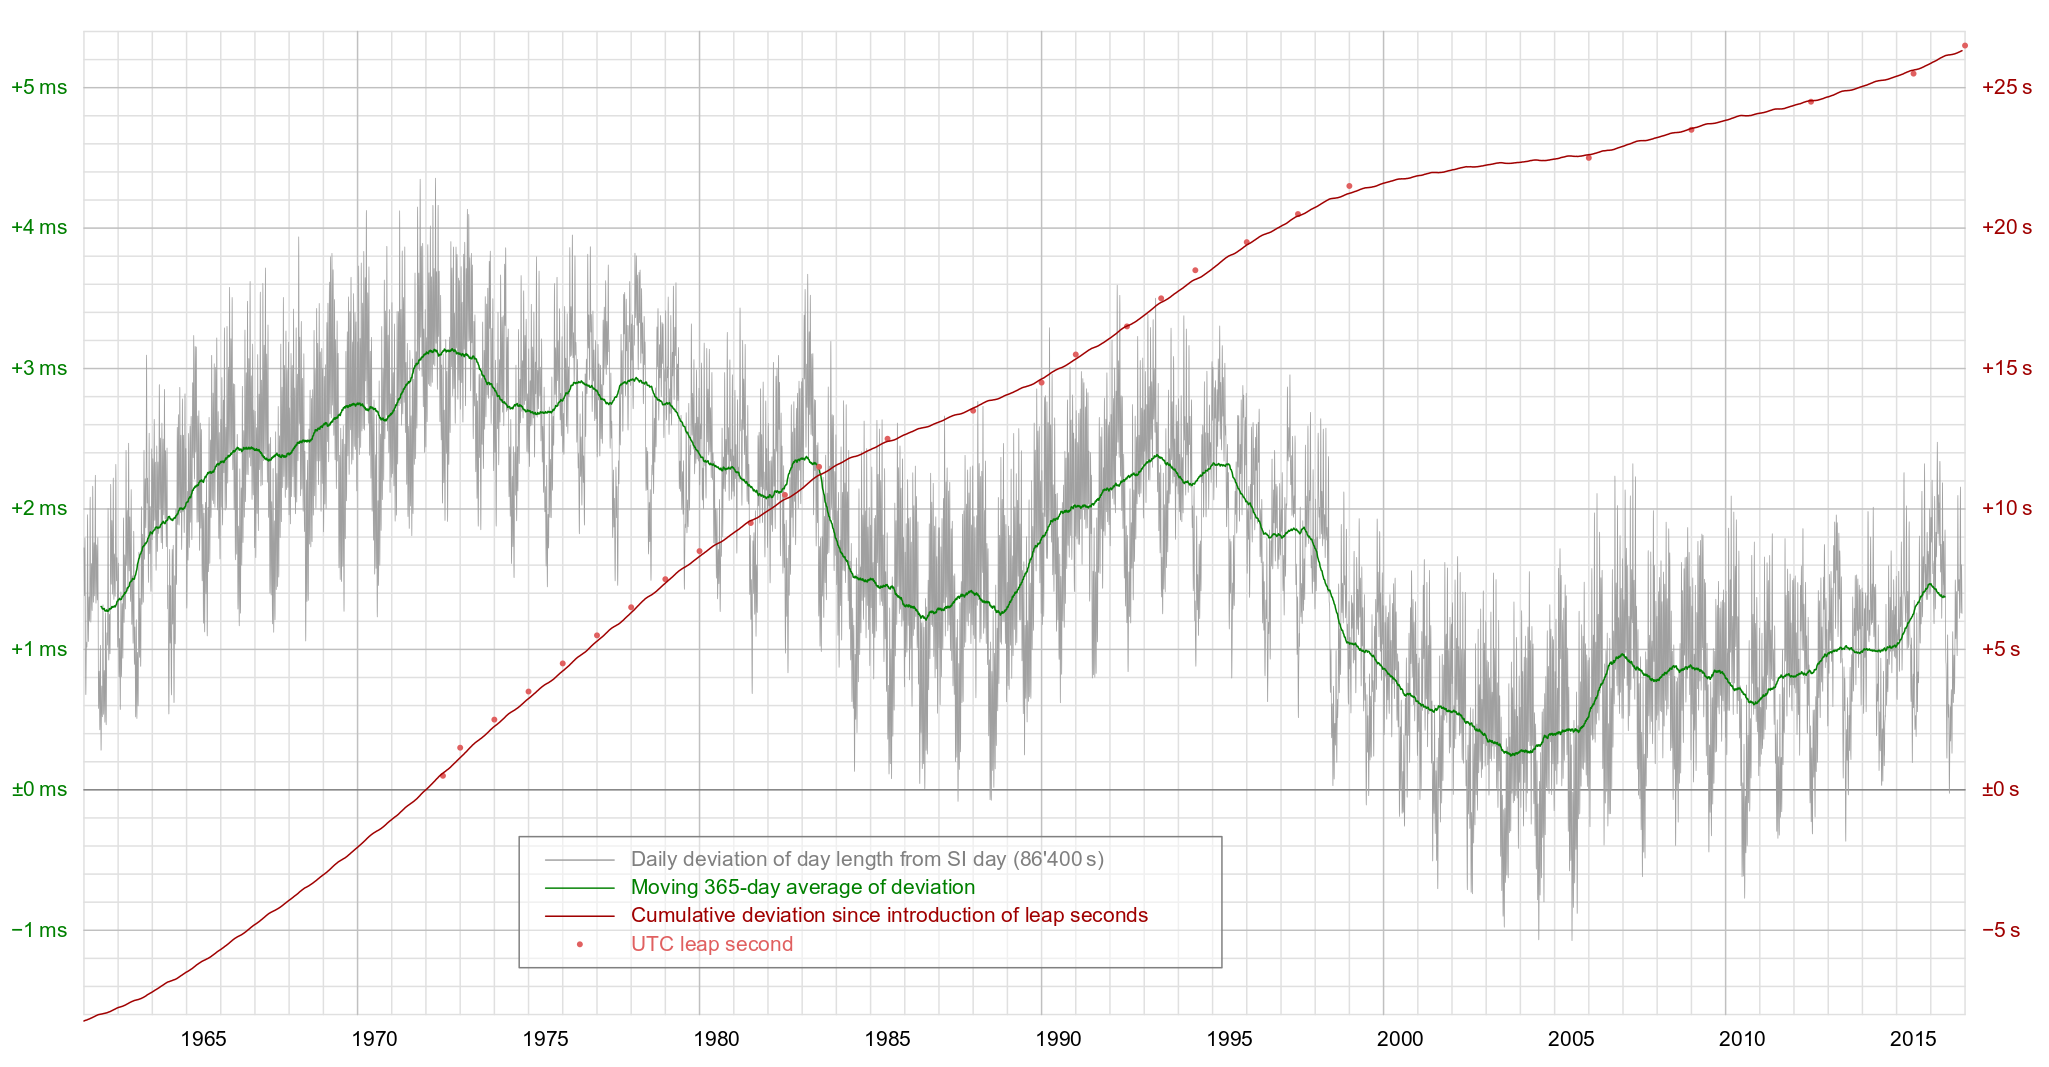
\includegraphics[width=1.0\textwidth]{figures/leap_second.png}
	\caption{Deviation of day length from SI day}
	\label{fig:leap_second}
	% https://upload.wikimedia.org/wikipedia/commons/5/5b/Deviation_of_day_length_from_SI_day.svg
\end{figure}

A leap second is a one-second adjustment that is occasionally applied to Coordinated Universal Time (UTC) to keep the difference with the mean solar time (UT1) within 0.9 second.\cite{ut} Without such a correction UTC would drift away from UT1 caused by irregularities of Earth's rotation rate. Since this concept was implemented in 1972 there were 27 leap seconds added with the most recent one on December 31, 2016 at 23:59:60 UTC.

In figure \ref{fig:leap_second} we can see the deviation of day length from SI day, the moving average, the cumulative deviation and the applied leap seconds.

\subsection{International Atomic Time}

The International Atomic Time (TAI\footnote{French abbreviation for Temps Atomique International.}) is a high-precision atomic coordinate time standard which is based on the notional passage of proper time on Earth's geoid.\cite{tai} It is the basis for Coordinated Universal Time (UTC). TAI can only differ from UTC by a multiple of a full second as a result of the definition of UTC.



\chapter{Method}
\label{ch:method}
Clock synchronization of multiple devices requires at least one time source to provide the ground truth. The goal of the synchronization is to get the target's clock as close as possible to the one of the source.

\section{General}

We can distinguish between two basic transmission methods: broadcast and client synchronization. Some protocols like PTP are a mixture of both.

\subsection{Broadcast synchronization}

The easiest method to synchronize time is to broadcast it periodically over a specific media, like radio or wire. This method is widely distributed across different devices. Some examples are: wristwatches, home weather stations, televisions and phones. This is analogous to a time report on the radio.

The broadcast synchronization method relies on the transmission delay of the time signal. The client has to believe the received time and doesn't know when it was originally sent. To keep the error small the transmission technology has to provide a certainty about the signal delay. For example Ethernet networks do not provide such a certainty. A "current time" packet could be sent over multiple network nodes which buffer it for some time and forward it afterwards. This could theoretically cause a delay not bound to a specific maximum.

One-way communications can only provide this method of time synchronization. Examples are DVB, GPS and radio clock.

\subsection{Client synchronization}

With this method, the client has the full control of the time synchronization process. He can query different servers and decide whom to trust or not. The client is also able to measure the round-trip time.

One downside of this method is that the network traffic scales with the number of clients. While the broadcast synchronization approach always has the same network load.

A popular example is NTP, while PTP is a combination of both: broadcast and client synchronization.

\section{Network Time Protocol}

The Network Time Protocol (NTP) synchronizes clocks of different devices over packet-switched, variable-latency networks.\cite{mills_2010} It is in operation since about 1985 and therefore one of the oldest Internet protocol in use. NTP was designed by David L. Mills at the University of Delaware.

NTP was invented to synchronize computer clocks within a few milliseconds of Coordinated Universal Time (UTC). It can achieve an accuracy within tens of milliseconds over the Internet or hundreds of microseconds in local area networks. Errors are caused by asymmetric routes and network congestion which results in 100 ms or more offset.

Usually the protocol is used in a client-server topology, but can also be used in a peer-to-peer relationship. Both peers would consider the other as a potential time source. The NTP daemon sends and receives timestamps over the User Datagram Protocol (UDP) on port 123. NTP could also be used to broadcast or multicast timestamps, while clients passively listen to updates from the server. The protocol also supplies warnings for any impending leap second adjustments. NTP does not cover any information about local time zones or daylight saving time.

The current version of the protocol is 4 (NTPv4), which is documented in RFC 5905 and backward compatible to version 3.

\subsection{Clock strata}

\begin{figure}[tb]
	\centering
	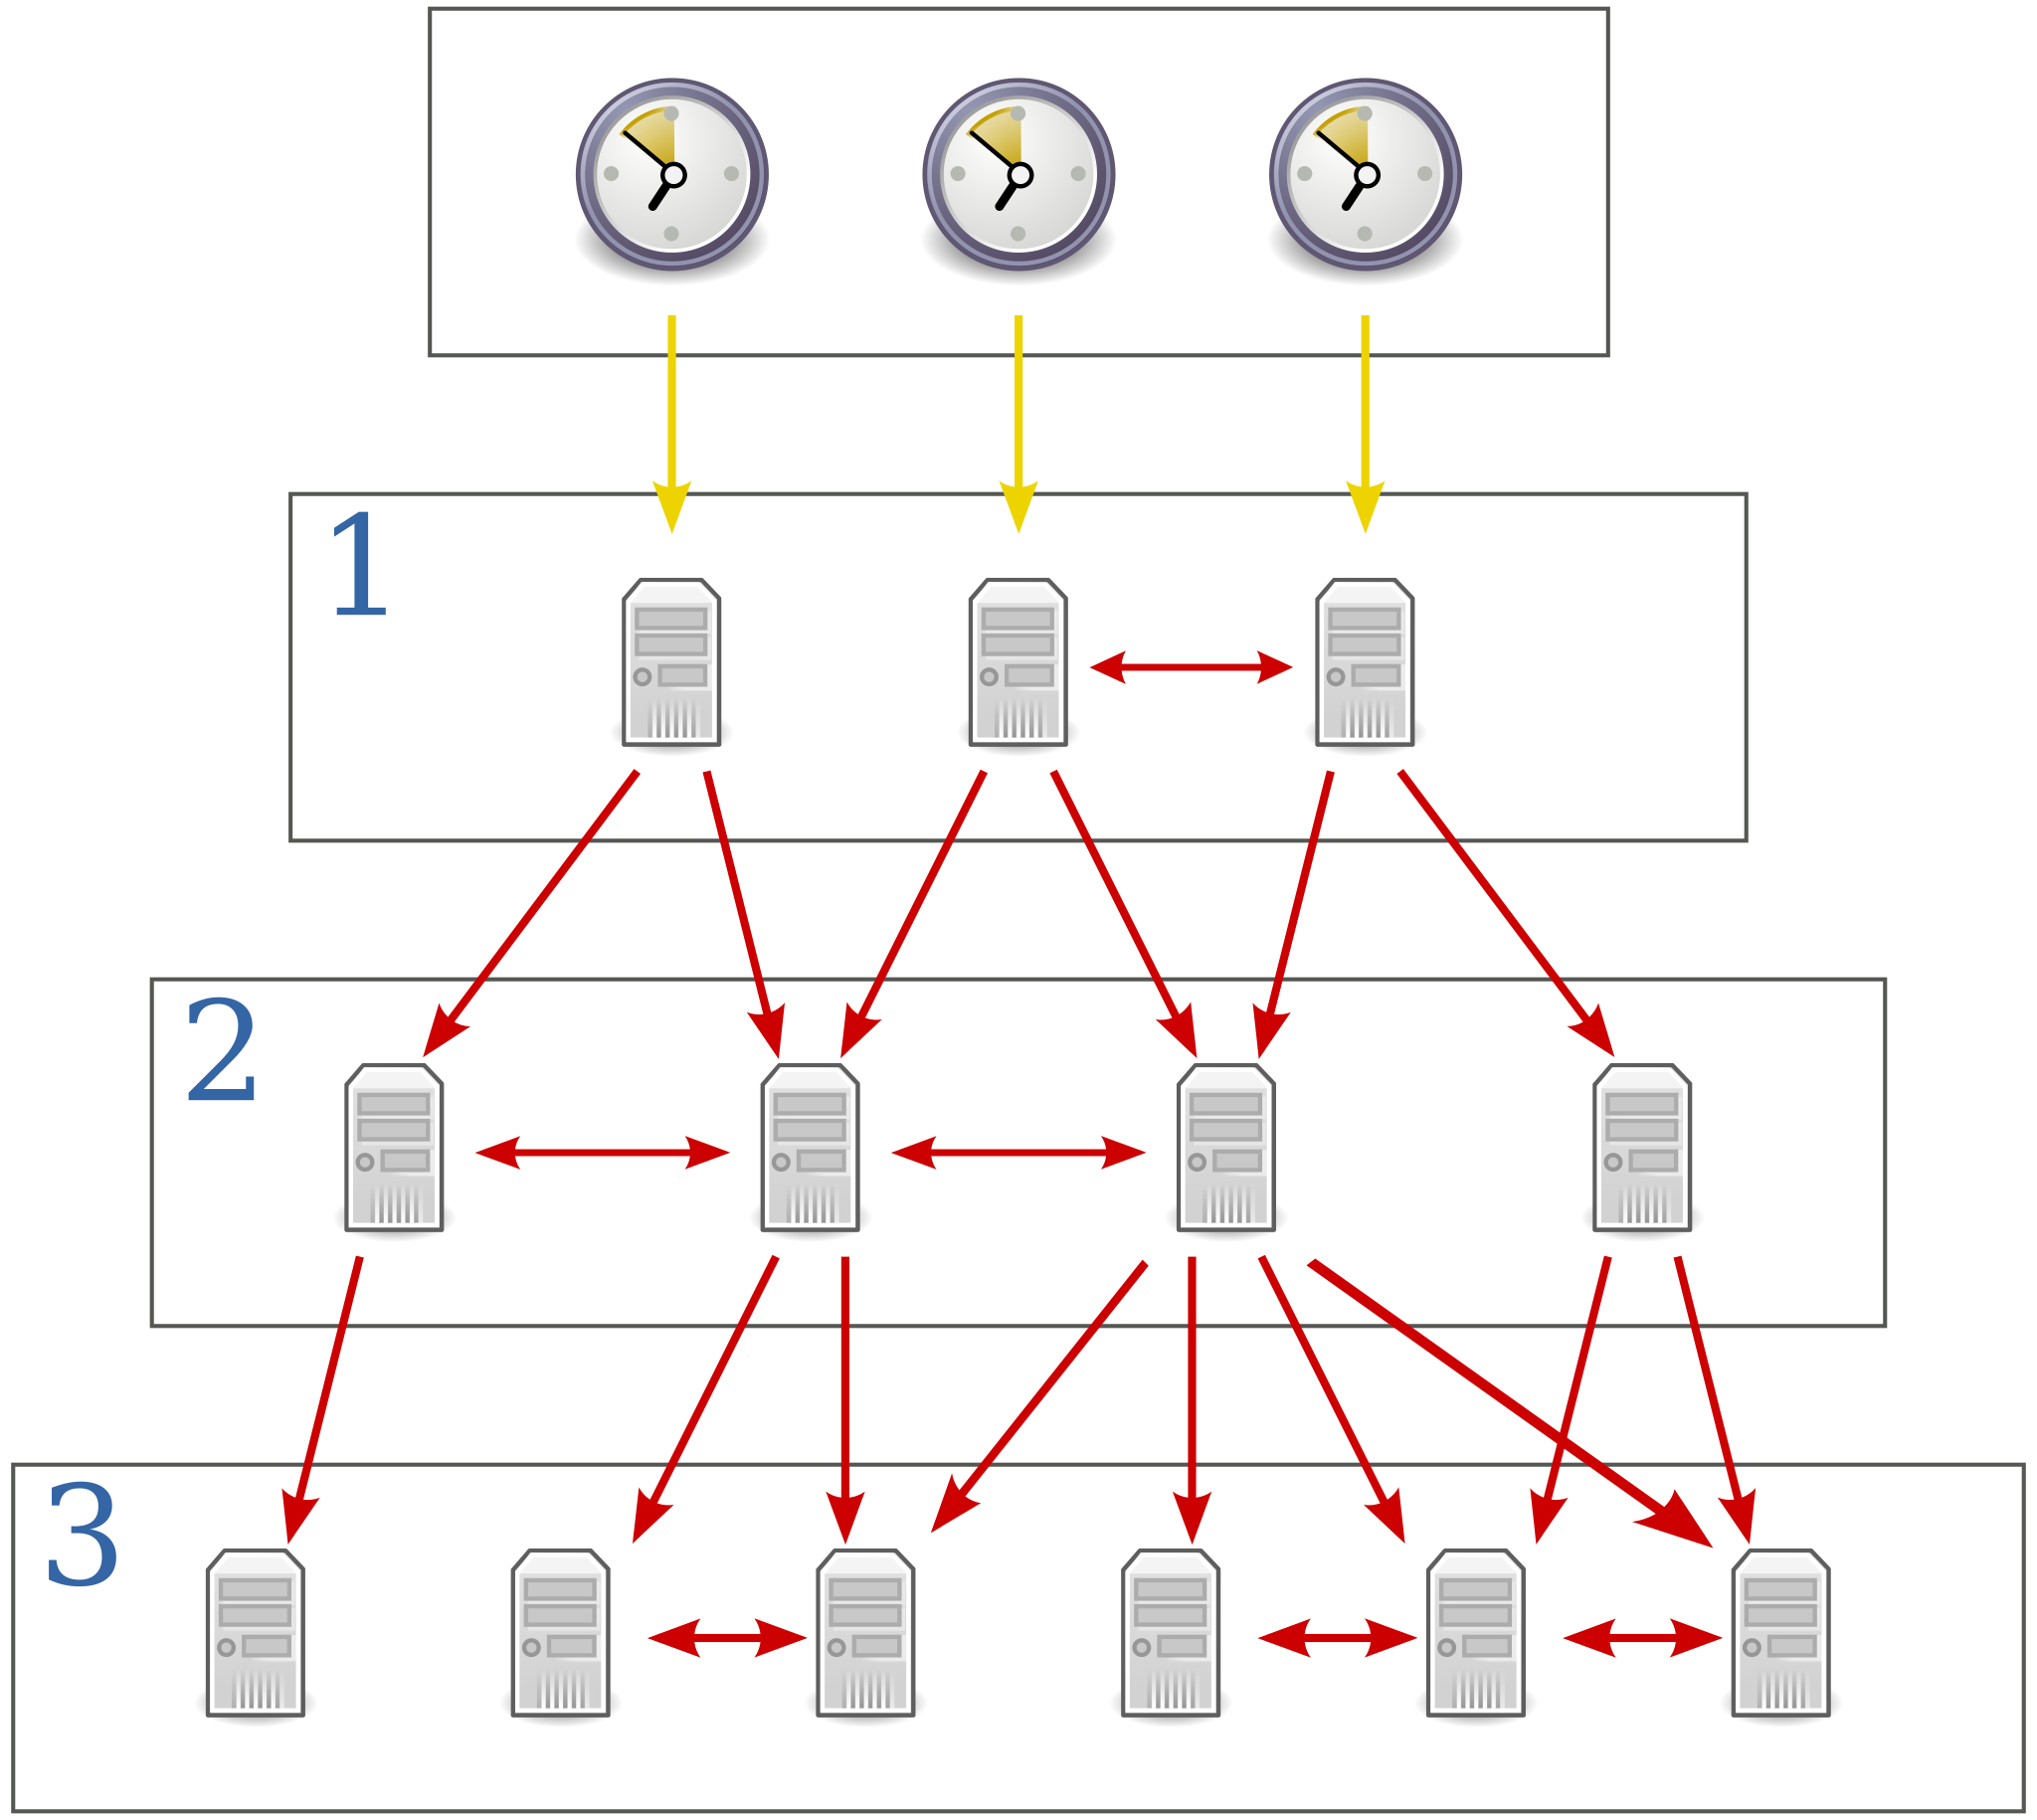
\includegraphics[width=0.7\textwidth]{figures/ntp_strata.png}
	\caption{Example of a NTP topology. The yellow arrows indicate a direct connection and the red ones a network connection.}
	\label{fig:ntp_strata}
	% https://upload.wikimedia.org/wikipedia/commons/c/c9/Network_Time_Protocol_servers_and_clients.svg
\end{figure}

NTP has a hierarchical structure of time sources. The different levels are called "stratum" and have a number from 0 to 16 assigned. This number represents the distance to the reference clock and is also used to prevent cyclical dependencies. The stratum should not be confused with the quality of the clock since this is not always true. There are stratum 3 servers providing higher quality than stratum 2 servers caused by lower latency for example. Stratum 16 indicates a unsynchronized device.

Stratum 0 devices are high-precision clocks, like atomic, GPS or other radio clocks. Usually they generate a pulse per second signal, which interrupts a connected computer to pickup the timestamp. Stratum 0 is also known as the reference clock.

Stratum 1 devices are computers which are synchronized to a stratum 0 device within microseconds. They maybe also connected to other stratum 1 servers for backup and sanity checking.

Figure \ref{fig:ntp_strata} shows an example of a logical NTP topology.

\subsection{Timestamps}

The NTP timestamp is 64 bits long and consists of a 32 bit seconds and a 32 bit fractional seconds part. That means it can represent about 136 years divided by a step size of about 233 picoseconds. NTP's zero in time is January 1, 1900 at 00:00:00 UTC, therefore the first roll will be on February 7, 2036.

Future versions of NTP may bring a 128 bit timestamp, with a 64 bit seconds and a 64 bit fractional seconds part. NTP inventor Mills said "the 64 bit value for the fraction is enough to resolve the amount of time it takes a photon to pass an electron at the speed of light. The 64 bit second value is enough to provide unambiguous time representation until the universe goes dim".

\subsection{Algorithm}

\begin{figure}[tb]
	\centering
	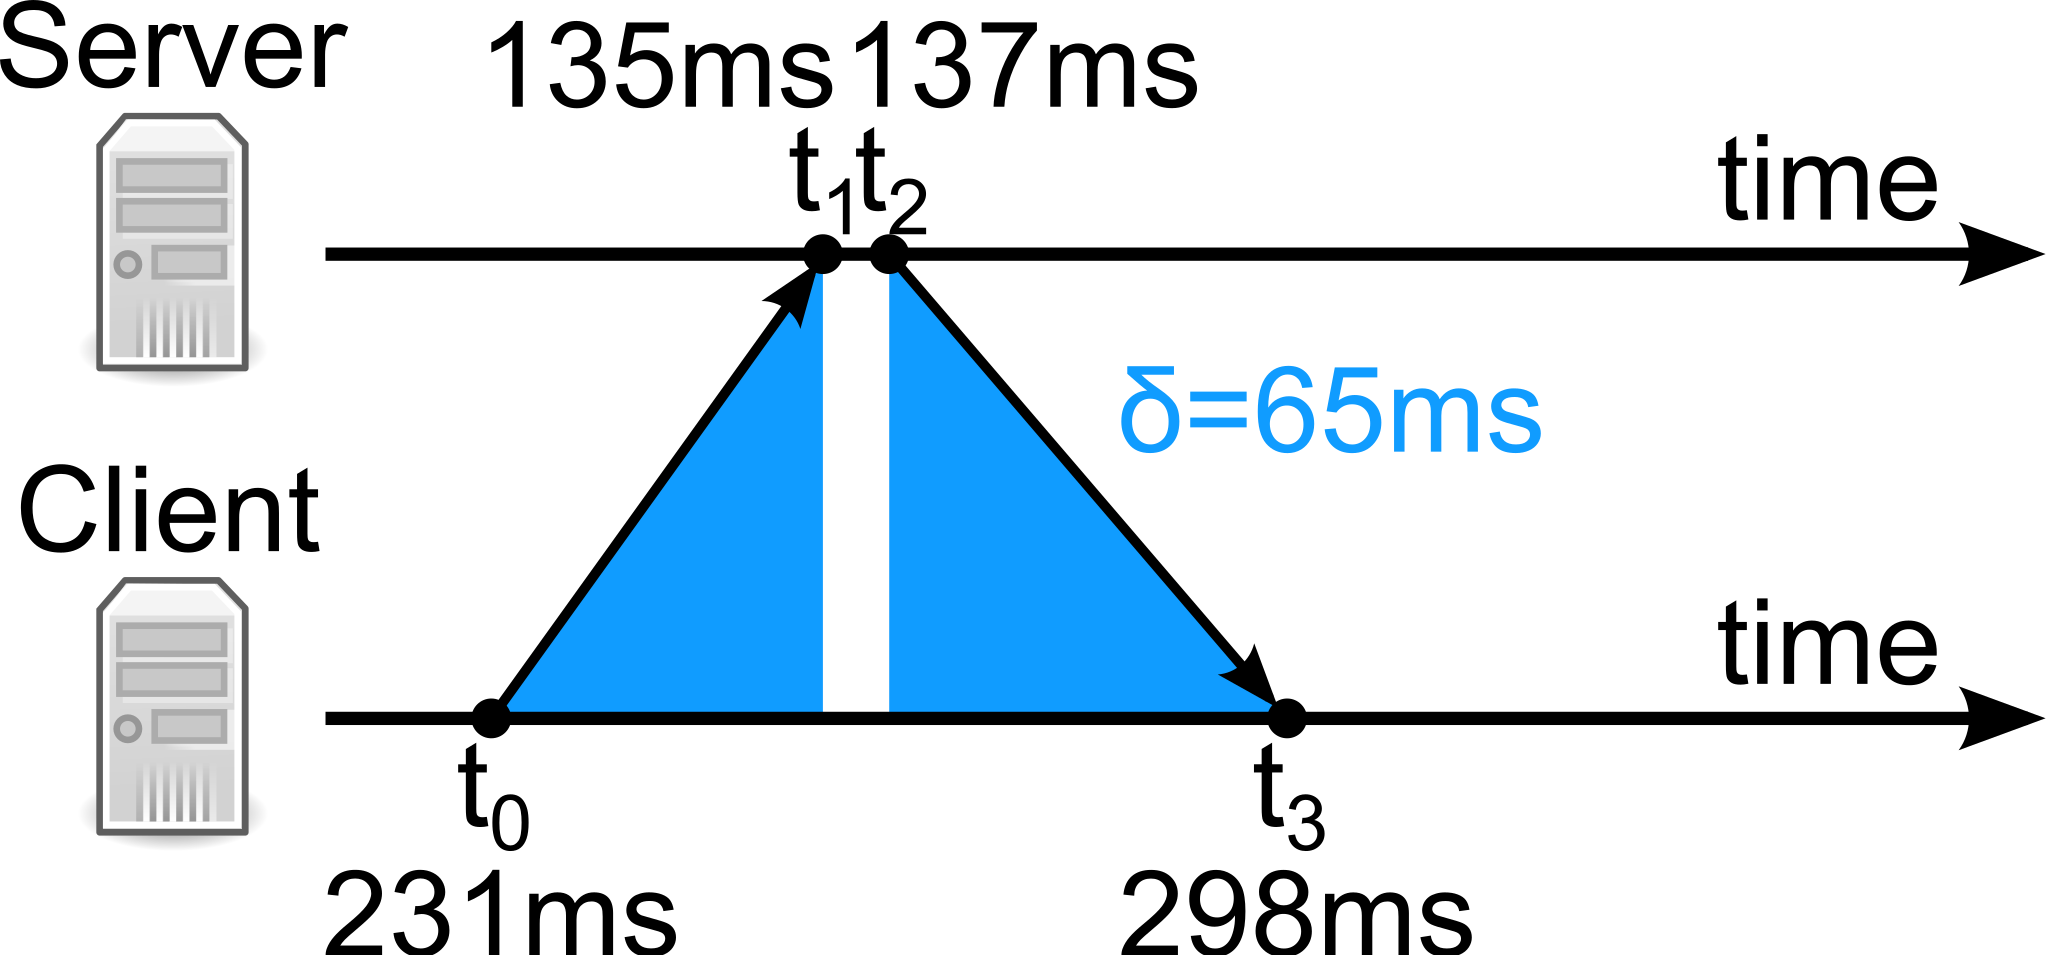
\includegraphics[width=0.7\textwidth]{figures/ntp_algorithm.png}
	\caption{Measurement process of the different timestamps}
	\label{fig:ntp_algorithm}
	% https://upload.wikimedia.org/wikipedia/commons/8/8d/NTP-Algorithm.svg
\end{figure}

With NTP the client has the full control of the synchronization process. It can poll different servers on diverse networks to synchronize its clock. As we can see in Figure \ref{fig:ntp_algorithm}, the client has 4 timestamps after such a poll. He can then calculate the time offset θ and the round-trip delay δ.

\[ \theta = \frac{(t_1 - t_0) + (t_2 - t_3)}{2} \]
\[ \delta = (t_3 - t_0) - (t_2 - t_1) \]

With:
\begin{description}
    \item[t_0] as the client's timestamp of the request packet transmission
    \item[t_1] as the server's timestamp of the request packet reception
    \item[t_2] as the server's timestamp of the response packet transmission
    \item[t_3] as the client's timestamp of the response packet reception
\end{description}

After the measurement, θ and δ are passed through filters. They are subjected to statistical analysis, outliers are discarded and the time offset is estimated. A feedback loop adjusts the clock frequency to reduce the offset gradually.

The algorithm assumes that both incoming and outgoing routes for server and client are symmetrical in regard to their delay. If this is not the case, there will be a systematic error of half the difference between client-server and server-client transmission delay.

\section{Precision Time Protocol}

Like NTP, the Precision Time Protocol (PTP) is used to synchronize clocks over packet-switched networks.\cite{eidson_2005,eidson_2006} But PTP promises higher clock accuracy, like sub-microsecond range on LANs. It was published 2002 in the IEEE 1588-2002 standard with the name "Standard for a Precision Clock Synchronization Protocol for Networked Measurement and Control System". The title already suggests that it could fit the needs of "Public Devices" very well. Later in 2008 the improved version PTP V2 was released in IEEE 1588-2008 which is backward compatible and improves accuracy, precision and robustness.

"IEEE 1588 is designed to fill a niche not well served by either of the two dominant protocols, NTP and GPS. IEEE 1588 is designed for local systems requiring accuracy beyond those attainable using NTP. It is also designed for applications that cannot bear the cost of a GPS receiver at each node, or for which GPS signals are inaccessible."\cite{eidson_book}

\section{Algorithm}

\begin{figure}[tb]
	\centering
	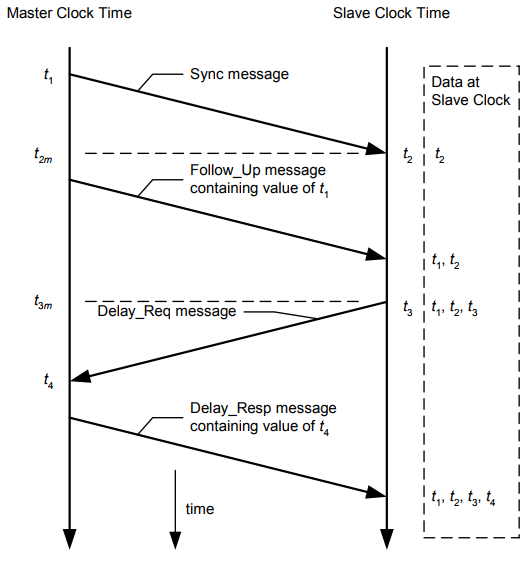
\includegraphics[width=0.7\textwidth]{figures/ptp_algorithm.png}
	\caption{Measurement process of the different timestamps}
	\label{fig:ptp_algorithm}
\end{figure}

The master periodically broadcasts his current time $t_1$ as a \textit{Sync} message to the slaves like shown in Figure \ref{fig:ptp_algorithm}. Under IEEE 1588-2002 broadcasts are up to once per second. Under IEEE 1588-2008, up to 10 per second are permitted. The slaves record the timestamp $t_2$ on receiving the \textit{Sync} message.

The \textit{Follow\_Up} message is optionally. Not all masters have the ability to provide an accurate timestamp right at sending the \textit{Sync} message. With common hardware and OS the best estimation of $t_1$ is right after the transmission is complete. This limitation leads the master to send the \textit{Follow\_Up} message to propagate $t_1$.

The slave continues with a \textit{Delay\_Req} message and keeps the transmission timestamp $t_3$. This is necessary to measure the individual round-trip time and to accurately synchronize to the master. After receiving the \textit{Delay\_Req} message and taking the timestamp $t_4$, the master responds with a \textit{Delay\_Resp} message and $t_4$.

After this procedure the slave has recorded the timestamps $t_1$, $t_2$, $t_3$ and $t_4$ which are necessary for calculating the offset from the master.

\[ o = \frac{(t_2 - t_1) + (t_3 - t_4)}{2} \]

The offset is then used to correct the slave by this amount to bring it into agreement with their master.

Like NTP, the offset and timestamps can further be passed through filters and subjected to statistical analysis. A feedback loop adjusts the clock frequency to reduce the offset gradually.

A few assumptions are made. First, the exchange of messages happens so fast that the measured offset can be considered as constant in between. Another assumption is, like with NTP, that the exchange has a symmetrical delay in both directions. Finally, it is assumed that timestamps can be measured accurately on sending and receiving messages. The resulting accuracy of PTP depends on how true these assumptions are in reality.

\section{Global Positioning System}

The Global Positioning System (GPS) is a global navigation satellite system (GNSS) set up to provide location and time information all around the world under all weather conditions.\cite{gps_sps,gps_waas} To do so, it needs an unobstructed line of sight to four or more GPS satellites. It has no further dependencies of any cellular or internet connection, but can be enhanced by those. The system was created by the US government, which maintains it and makes it freely accessible to anyone.

Each satellite transmits its position and time to the earth. A GPS device that receives messages from at least 4 different satellites is able to calculate its position.

As GPS is very time sensitive, each satellite carries a very stable atomic clock which is synchronized with another one and ground clocks. The clock drift is corrected every day.
These very accurate clocks can be used to synchronize a computer's clock within nanoseconds.



\chapter{Implementation}
\label{ch:impl}
Since the "Public Devices" should be cheap, single-board computers were chosen as the target system. The most widely distributed one is the Raspberry Pi. It has the benefit of a large community and Linux mainline support. This makes it easy to maintain and provides a trustful platform to implement such a measurement system.

\section{Raspberry Pi 3}

\begin{figure}[tb]
	\centering
	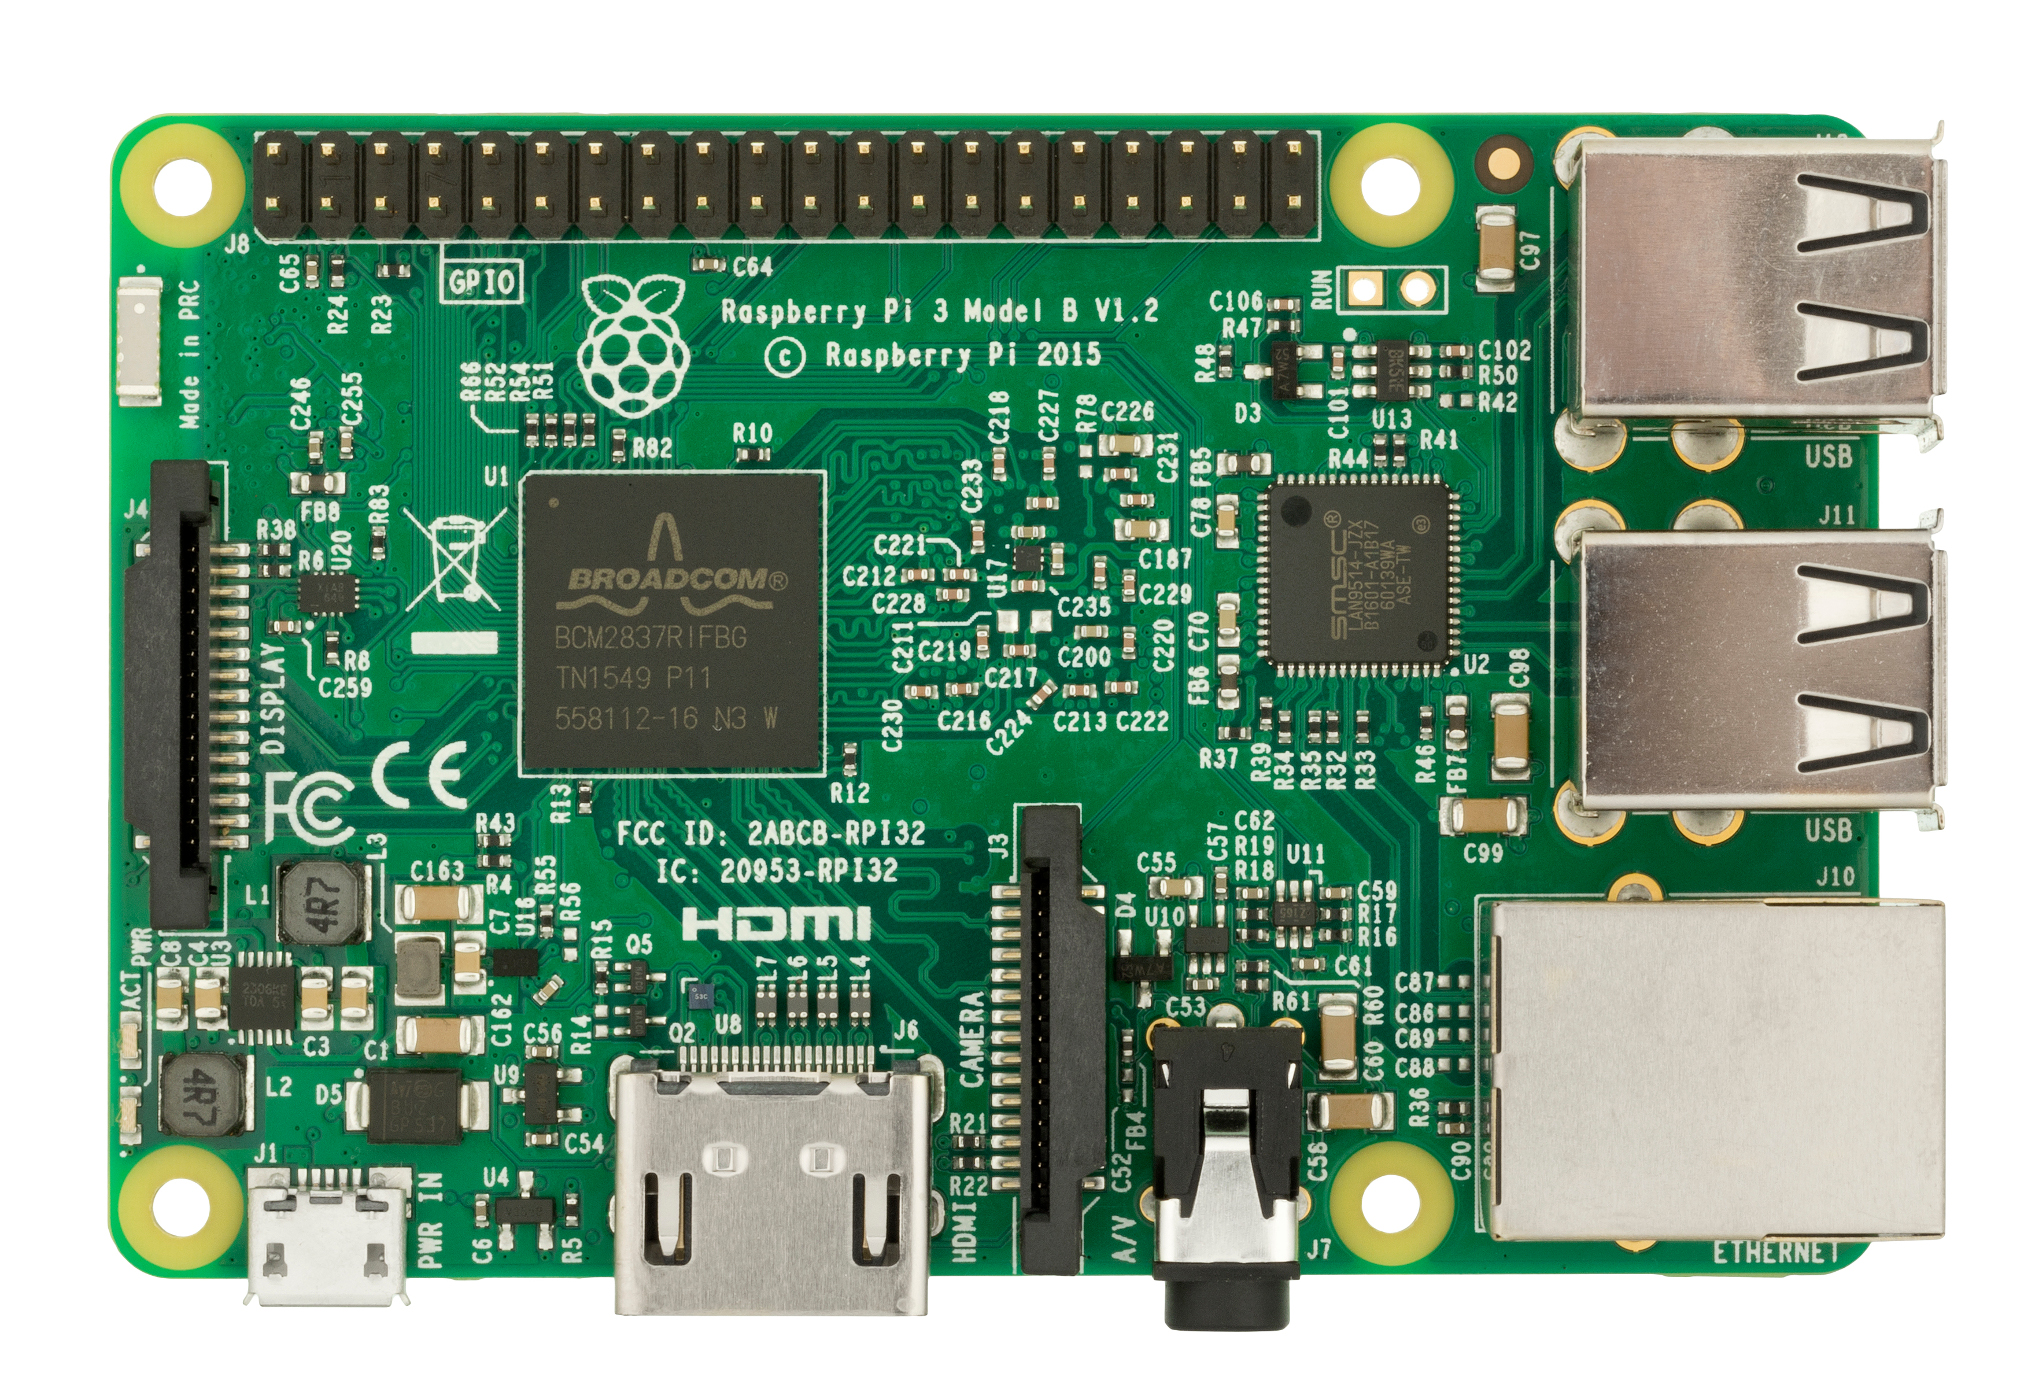
\includegraphics[width=0.7\textwidth]{figures/rpi3.jpg}
	\caption{Raspberry Pi 3 Model B}
	\label{fig:rpi3}
	% https://upload.wikimedia.org/wikipedia/commons/e/e6/Raspberry-Pi-3-Flat-Top.jpg
\end{figure}

The Raspberry Pi is a single-board computer with the size of a credit card. It was developed in the United Kingdom by the Raspberry Pi Foundation and was made for schools and developing countries to promote teaching the basics of computer science. It is a very flexible platform for prototyping and an easy to use hardware component ready to be programmed. It provides GPIOs and supports the serial bus technologies I²C and SPI.

There are a few different models of the Raspberry Pi, but all of them feature a Broadcom system on a chip (SoC). It includes an ARM compatible central processing unit (CPU) and an on-chip graphics processing unit (GPU). Each model provides a SD card slot to store the operation system and user specific data, like programs.

Further specifications:
\begin{itemize}
\item CPU with 1.2 GHz quad core
\item 1 GB RAM
\item 4 USB Ports
\item Ethernet
\item Wi-Fi 802.11n and Bluetooth
\end{itemize}

The most popular Linux distribution used with the Raspberry Pi is the Debian based Raspbian. Other available operating systems are Ubuntu, Windows 10 IOT Core, and RISC OS.

\section{Adafruit Ultimate GPS Breakout v3}

\begin{figure}[tb]
	\centering
	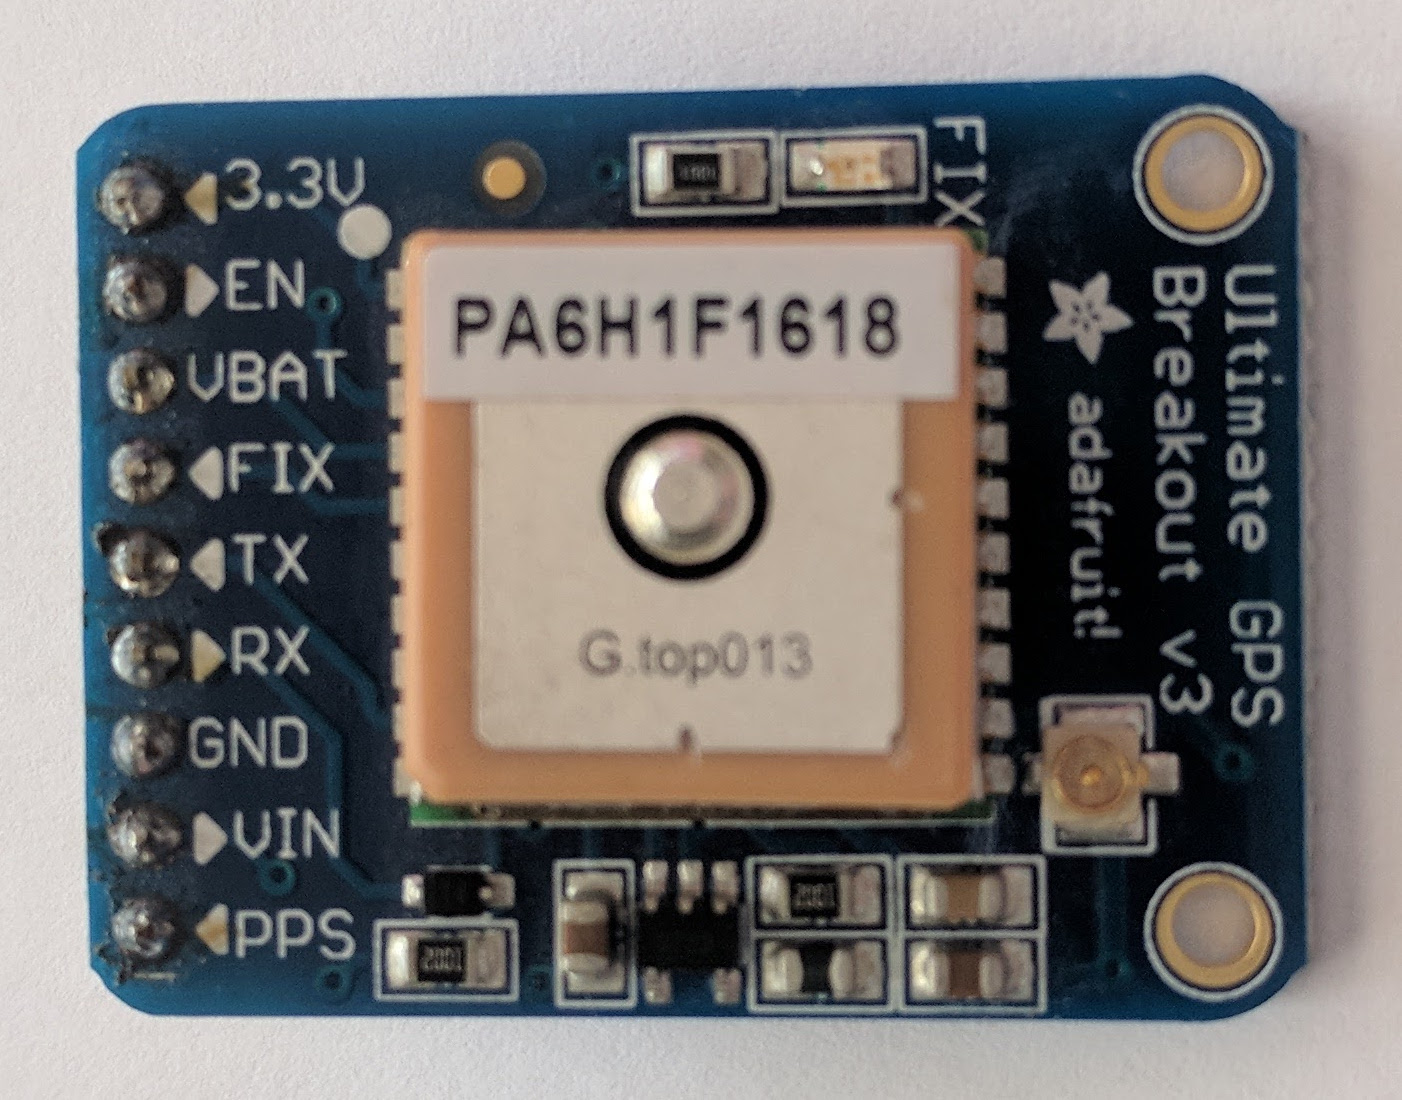
\includegraphics[width=0.7\textwidth]{figures/gps.jpg}
	\caption{Adafruit Ultimate GPS Breakout v3}
	\label{fig:gps}
\end{figure}

The “Adafruit Ultimate GPS Breakout v3” comes with a MTK3339 chipset and provides an easy to use and reliable GPS interface. The serial port transmits the position and satellite data in common NMEA sentences while an additional PPS output emits a digital pulse on each UTC second.

Further specifications:
\begin{itemize}
\item Satellites: 22 tracking, 66 searching
\item Patch Antenna Size: 15mm x 15mm x 4mm
\item Update rate: 1 to 10 Hz
\item Position Accuracy: < 3 meters (all GPS technology has about 3m accuracy)
\item Velocity Accuracy: 0.1 meters/s
\item Vin range: 3.0-5.5VDC
\item Output: NMEA 0183, 9600 baud default, 3V logic level out, 5V-safe input
\item PPS output on fix
\item RTC battery-compatible
\end{itemize}

\section{Linux}

Linux as an operating system kernel was first released on September 17, 1991 by Linus Torvalds. The kernel is the defining component of Linux. The operating system (OS) is a Unix-like and mostly POSIX-compliant system. It is assembled with the idea of free and open-source software development and distribution.

Linux has a monolithic kernel which means that the entire operating system is working in a separated memory section, called kernel space, and is the only software running in supervisor mode. This concept is different to other architectures in the way that only the kernel provides a high-level virtual interface to the device hardware. Modifications like additional drivers can be inserted as kernel modules.

Linux is by far the most common operating system for embedded devices. Examples are: network devices, smart TVs, security cameras, smartphones.

Nowadays Linux is supported by major companies like Dell, IBM, HP and Oracle.

\subsection{Kernel modules}

A kernel module is a piece of software that can be loaded to the kernel on demand. This is the only way to insert custom software to the kernel space and running it in supervisor mode (except modifying the kernel source or utilizing exploits).

Usually, kernel modules are used as drivers to integrate hardware which is not supported by the kernel out of the box. This keeps the kernel image small and ready for devices with small resources.

Such a module offers an easy way to extend the functionality of the kernel without adopting the kernel source itself and then compiling it together. That saves a lot of time, since Linux kernel compilation can be a heavy task. Besides that, a kernel module can be loaded and tested on runtime, while the kernel itself can only be loaded on startup.

Usually kernel modules reside in the /lib/modules/<kernel\_version>/kernel/ directory and have a .ko extension.

\subsection{PREEMPT\_RT patch}

Written and supported by Luotao Fu and Robert Schwebel, PREEMPT\_RT is a patch for the Linux kernel to enable hard real-time capabilities while the standard Linux kernel only provides soft real-time capabilities with no guarantees for hard timing deadlines. Since the patch became more and more usable and is mainline integratable, significant parts have already leaked into the Linux kernel.

\subsection{Kernel compilation}

In order to use the PREEMPT\_RT patch, we have to compile the whole kernel with it. To compare the difference to the standard kernel, the same kernel version without the patch should be compiled too.

Since the kernel takes hours to compile on the Raspberry Pi itself it is recommended to compile it on a faster device. Usual workstations have a different CPU architecture than ARM, which leads us to cross-compilation. There is a toolchain on GitHub hosted by the Raspberry Pi Foundation for such cases.

You can find the kernel compilation steps in Appendix A.

\section{GPS setup}

A small setup is required to use the Adafruit GPS module on Linux. There is a serial interface to transmit the NMEA sentences and a digital output for the pulse per second (PPS) signal. The Raspberry Pi provides a serial interface directly at its pinout. Usually it is used to provide shell access to the OS but can also be configured to act as an usual tty device. A kernel module handles the desired GPIO pin and creates a pps device which can then be used by the NTP daemon.

You can find the kernel GPS setup in Appendix C.

\section{Tools}

\subsection{Cyclictest}

Cyclictest was used as a benchmark for the different kernels. The results can be found in the "Measurements" section. It has a simple measurement concept and provides useful results to decide the target OS. A pseudocode is shown in Listing \ref{lst:cyclictest}.

\begin{lstlisting}[label=lst:cyclictest, language=C, caption=Cyclictest pseudocode]
clock_gettime(&now)
next = now + interval
while (!shutdown) {
  clock_nanosleep(&next)
  clock_gettime(&now)
  diff = now - next
  # update stat -> min, max, total latency, cycles
  # update the histogram data
  next += interval
}
\end{lstlisting}

The description from the website\footnote{\url{https://wiki.linuxfoundation.org/realtime/documentation/howto/tools/cyclictest}} is:

\begin{displayquote}
Cyclictest is a high resolution test program originally written by Thomas Gleixner (tglx). A lot of people contributed to it later on and it is currently being maintained by Clark Williams and John Kacur. It is part of the test suite rt-tests.

The cyclictest runs a non real-time master thread (scheduling class SCHED\_OTHER) which starts a defined number of measuring threads with a defined real-time priority (scheduling class SCHED\_FIFO). The measuring threads are woken up periodically with a defined interval by an expiring timer (cyclic alarm). Subsequently, the difference between the programmed and the effective wake-up time is calculated and handed over to the master thread via shared memory. The master thread tracks the latency values and prints the minimum, maximum and average for the latency once the number of iterations specified is completed.
\end{displayquote}

\subsection{time-experiments}

A toolset providing the different measurement implementations, primarily written in Python. To increase accuracy some parts were moved to C and get called by the Python scripts. To receive GPIO interrupts as soon as possible, a kernel module was written. The whole source code and documentation can be found on GitHub.

\subsection{time-analysis}

A collection of filter and plot scripts in Python. All the measured data was processed with the help of these scripts. The source code and documentation can be found on GitHub.

\subsection{time-config}

A tool to simplify the clock synchronization setup. It supports NTP, PTP and GPS. It is also meant to simplify the autostart of the desired time synchronization process with a small configuration file. The source code and documentation can be found on GitHub.

\subsection{time-tools}

A small collection of bash scripts to simplify the measurement process. This includes loading the kernel module, invoking the measurement client and server, switching the kernel between standard and PREEMPT\_RT and tweaking the local clock.

\subsection{adjtimex}

This tool allows direct access to the kernel time variables. It can be used to tune the clock speed manually. For this project it was used to intentionally set the clock frequency too fast or too slow before a new synchronization process was initiated.



\chapter{Measurements}
\label{ch:measurements}
The major part of this thesis was to measure and compare the different synchronization methods and provide a selection basis. To get comparable results, the first step was to choose the hardware and OS for the measurement system. Since the hardware was already given by "Public Devices" with the Raspberry Pi 3 and Linux as the OS, the kernel was the last option to choose.

All measurements were taken under optimal conditions: no CPU load, no RAM load, no storage load, no network load.

\section{Setup}

A detailed installation of the measurement environment is described in Appendix D. The devices connected to a GPS module additionally require the setup described in Appendix C.
The measurements were done with three Raspberry Pis. All of them were connected over Ethernet and a switch. One of them has to transmit a measurement pulse over GPIO 3 to the others' GPIO 2 like described in the "Time vs time" section.

\section{Delays}

A measurement system should provide small latency to get a sharp resolution in time. The popular PREEMPT\_RT patch promises that and was the other option besides the mainline kernel. Both were compiled as described before and exchanged for the different measurements.
Another option to improve latency is to disable the dynamic clock speed of the CPU. This is intended to reduce the power draw in idle situations. But it will increase the latency since important measurement instructions may run on low clock speed in the first place before the kernel reacts to the rising CPU load.

We can divide the delay into different parts. It starts with the internal hardware clock, the OS and the measurement software. Further parts come from the hardware interface, the signal transmission and measurement instrument itself. The aim for this thesis is to minimize the OS delay and provide an overview of interface and transmission delays.

The system delay will tell us which kernel to choose. The accuracy of time synchronization is very much related to the underlying transmission method and provides a first estimation of the error. This error can then be minimized with statistical methods. The delay of the used transmission methods will give an overview.

\subsection{System delay}

The OS delay was measured with the tool cyclictest, which was described before.

\begin{figure}[H]
	\centering
	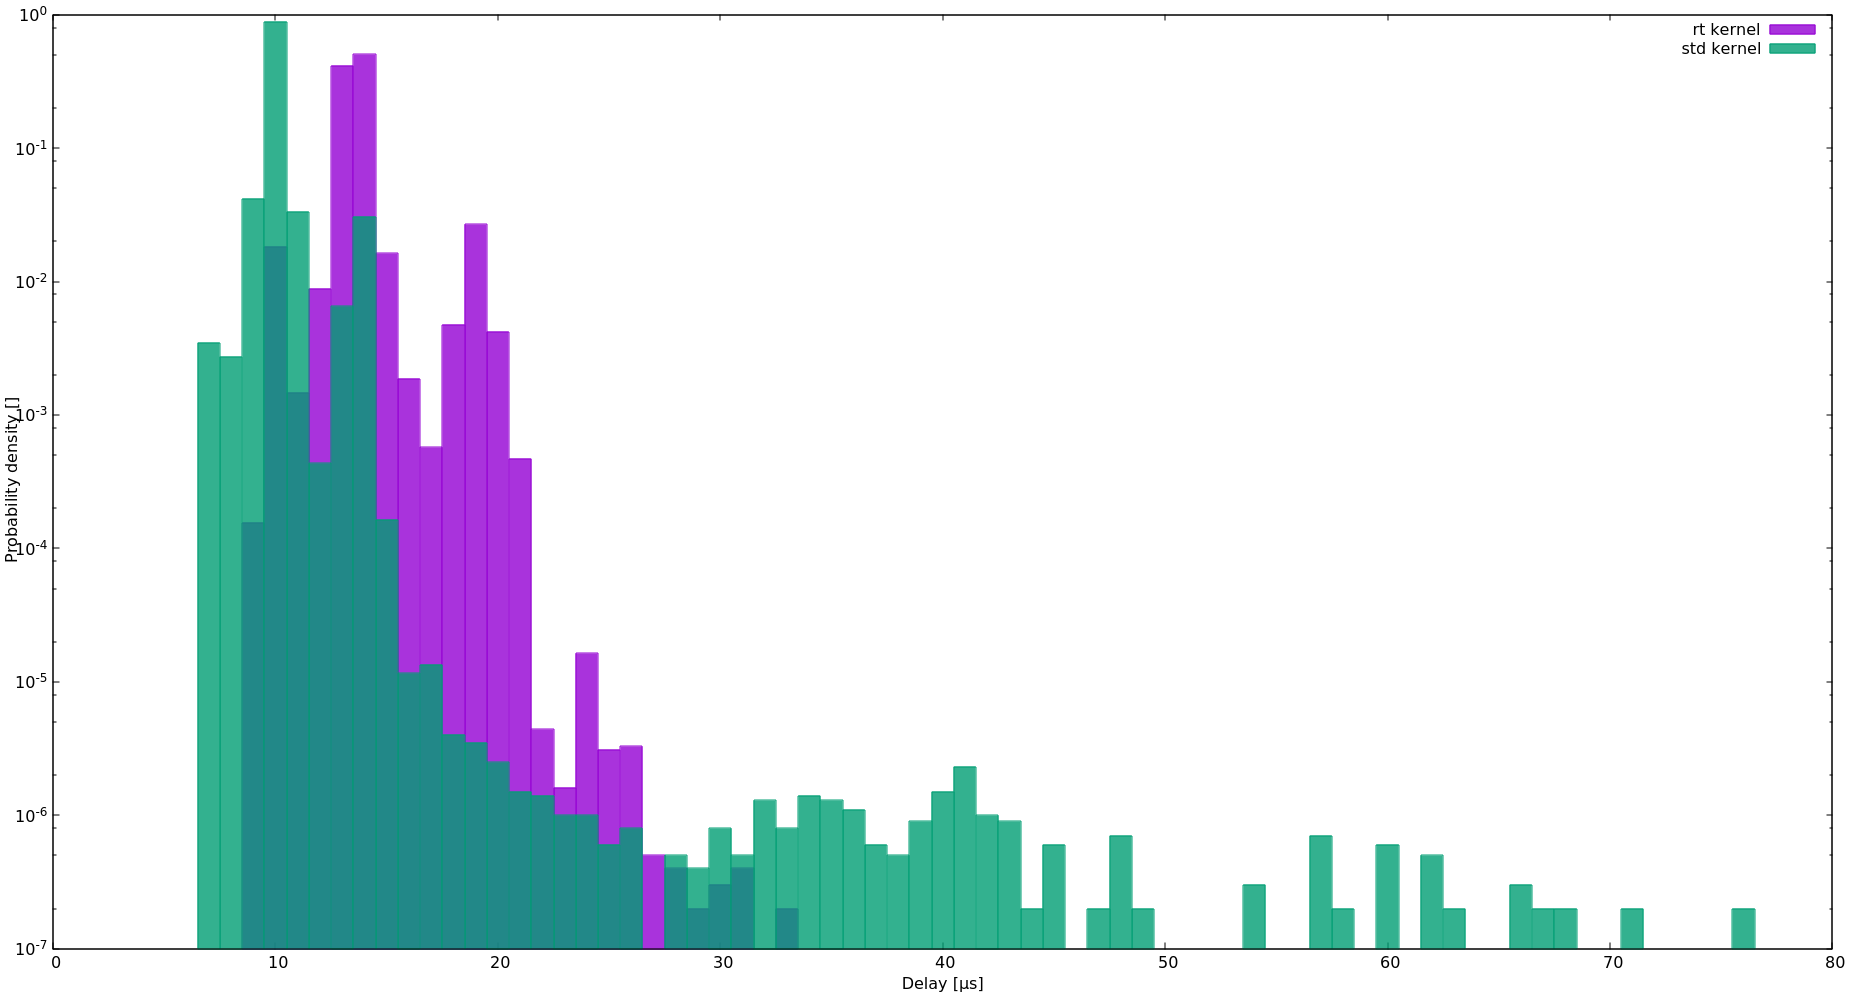
\includegraphics[width=1.0\textwidth]{figures/plot_system.png}
	\caption{System delay}
	\label{fig:plot_system}
\end{figure}

Figure \ref{fig:plot_system} is a plot of the probability density over the delay. Where "rt kernel" stands for the PREEMPT\_RT patched and "std kernel" for the mainline kernel.
As we can see, the PREEMPT\_RT patch gives us a better delimitation but the mainline kernel provides a higher peak with 88\% at 10 µs.

\begin{center}
    \begin{tabular}{ | l | r | r | r | }
    \hline
    \textbf{Target} & \textbf{Delay avg} [µs] & \textbf{Delay min} [µs] & \textbf{Delay max} [µs] \\ \hline
    rt & 13 & 9 & 37 \\ \hline
    std & 10 & 7 & 76 \\ \hline
    \end{tabular}
\end{center}

Issued command:

\begin{lstlisting}[language=bash]
rt-tests/cyclictest -m -t1 -p 99 -n -i 400 -l 10000000 -q -H 400
\end{lstlisting}

\subsection{GPIO delay}

The general-purpose input/output (GPIO) provides a general, easy to use and fast way to generate and process digital signals. Since the Adafruit GPS module has a pulse per second (PPS) signal output, we want to know how accurate this interface is.
To do so, two pins were connected together, one used as an output and the other as an input. Then the time difference between generating and receiving an impulse it is taken. This was repeated for a period of time to get a smooth delay distribution.

\begin{figure}[H]
	\centering
	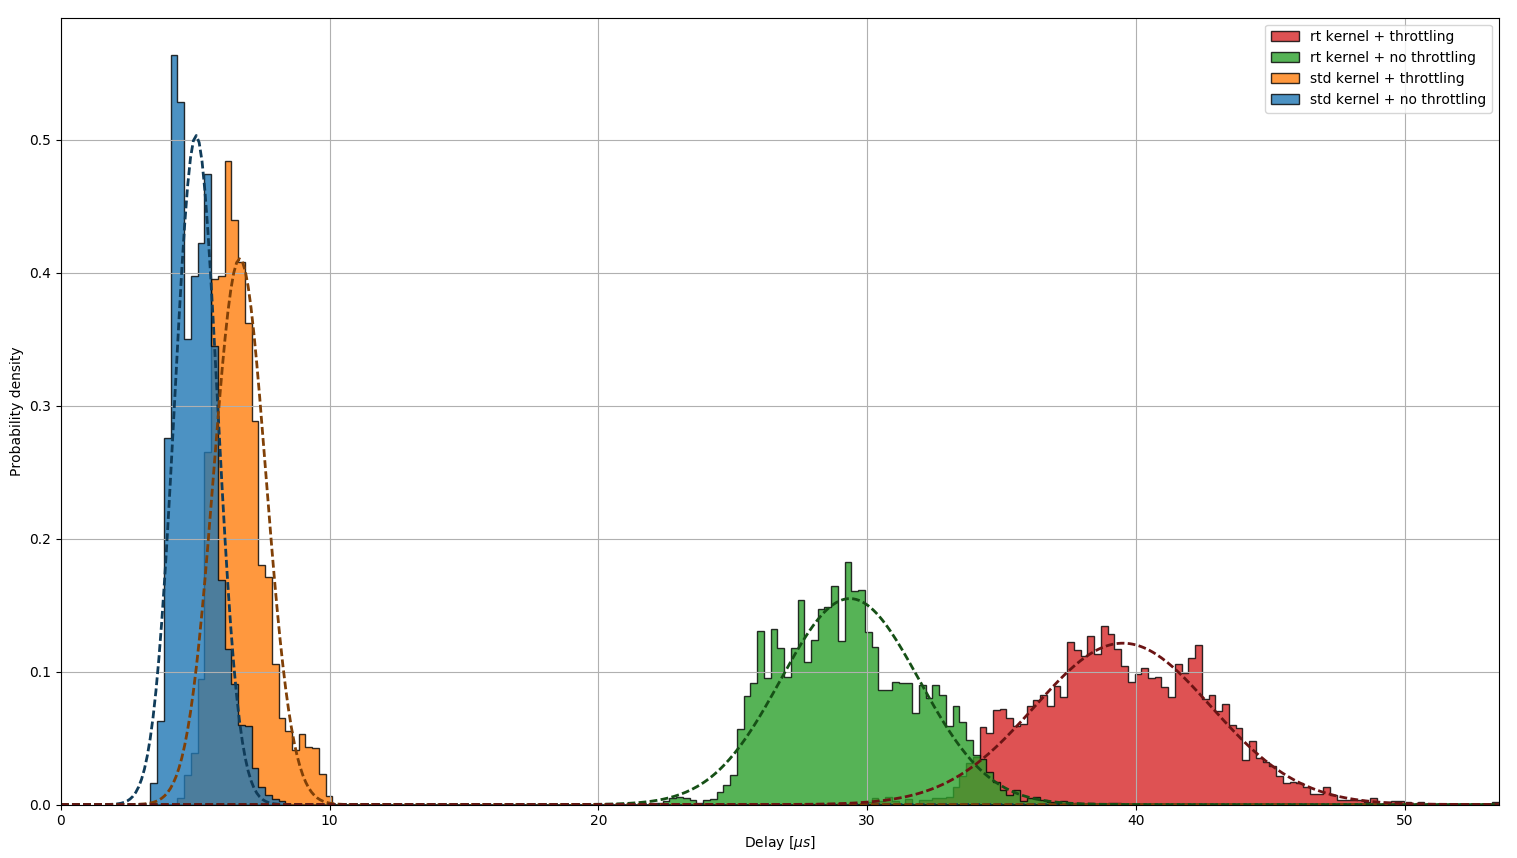
\includegraphics[width=1.0\textwidth]{figures/plot_gpio.png}
	\caption{GPIO delay}
	\label{fig:plot_gpio}
\end{figure}

The measured distributions are shown in Figure \ref{fig:plot_gpio}. Where "rt kernel" stands for the PREEMPT\_RT patch and "std kernel" for the standard mainline kernel. In addition, the CPU was configured to stay with a single frequency designated with "no throttling" and the default configuration with "throttling".
As we can see, configuring the Raspberry Pi to not adopt the CPU's frequency has a noticeable impact on the delay. The latency with the PREEMPT\_RT patch is not only about 6 times higher, but also more spread out. A wider distribution will also cause a higher error for a time synchronization method that relies on GPIO like GPS.

The enveloping gaussians are parameterized as the following:

\begin{center}
    \begin{tabular}{ | l | r | }
    \hline
    \textbf{Target} & \textbf{Delay} [µs] \\ \hline
    std kernel + no throttling & 5.0\pm 0.8 \\ \hline
    std kernel + throttling & 6.7\pm 1.0 \\ \hline
    rt kernel + no throttling & 29.4\pm 2.5 \\ \hline
    rt kernel + throttling & 39.5\pm 3.3 \\ \hline
    \end{tabular}
\end{center}

The static CPU frequency was configured by adding the following lines to /boot/config.txt:
\begin{lstlisting}[language=bash]
# static frequency
force_turbo=1
arm_freq=800
arm_freq_min=800
\end{lstlisting}

Issued commands:

\begin{lstlisting}[language=bash]
time-tools/measure-server -i 0.5 &
time-tools/measure-client 127.0.0.1 &
\end{lstlisting}

\subsection{Network delay}

The network delay is very important for NTP and PTP. The delay distribution gives a first estimation of the synchronization error. With the assumption that the delay is the same in both directions and it doesn't vary too much, the error can be reduced by statistical methods like described in the NTP and PTP chapter.

\begin{figure}[H]
	\centering
	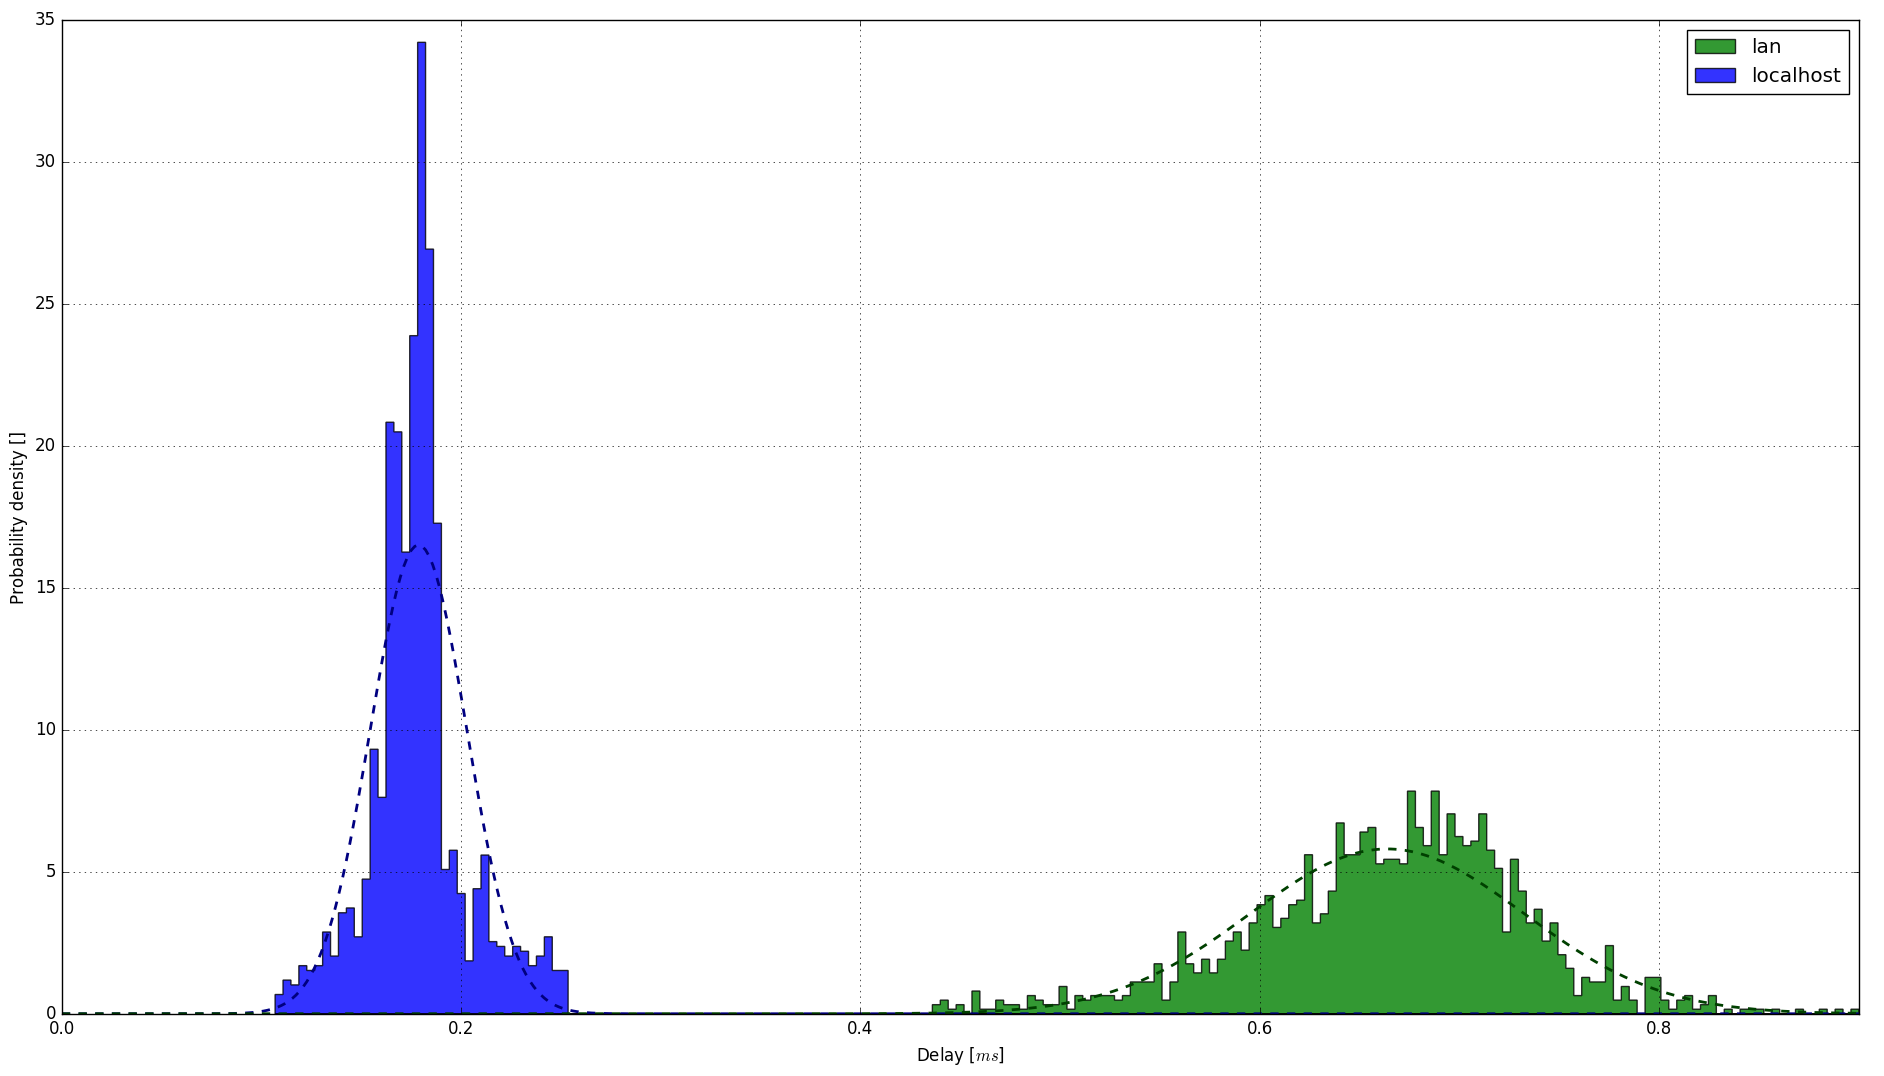
\includegraphics[width=1.0\textwidth]{figures/plot_network.png}
	\caption{Network delay}
	\label{fig:plot_network}
\end{figure}

The measured distributions are shown in Figure \ref{fig:plot_network}. The localhost measured to get an idea of what delay is caused by the OS itself. For a LAN attached device we get a similar distribution like "lan". It fits the gaussian distribution very well.

The enveloping gaussians are parameterized as the following:

\begin{center}
    \begin{tabular}{ | l | r | }
    \hline
    \textbf{Target} & \textbf{Delay} [ms] \\ \hline
    localhost & 179\pm 24 \\ \hline
    lan & 664\pm 69 \\ \hline
    internet & 25634\pm 213 \\ \hline
    \end{tabular}
\end{center}

Issued command:

\begin{lstlisting}[language=bash]
delay-icmp <host>
\end{lstlisting}

\subsection{NMEA delay}

Since the GPS module has two different transmission methods to emit a second, a calibration is required. While the PPS line gives us a single digital pulse when a UTC second has started, the serial connection tells us which second it was. The delay between those two can be measured and passed to the NTP daemon.

The delay was measured with: (435\pm 89) ms

Issued command:

\begin{lstlisting}[language=bash]
delay-nmea -s ~/time-experiments.c/nmea_pulse /dev/ttyS0 ~/time-experiments.c/pps_pulse /dev/pps0
\end{lstlisting}

\section{Time deviation}

The following measurements were taken to see the moving time offset of connected Raspberry Pis to a chosen norm. With the help of that we can visualize the process of time synchronization with a resolution of a few µs.

The three Raspberry Pis were called \textit{rpi1}, \textit{rpi2} and \textit{rpi3}. \textit{rpi1} was chosen to be the server and therefore the norm to compare to. The two GPS modules were connected to \textit{rpi1} and \textit{rpi2}. In order to measure the time accurately the server is connected to all his clients with per GPIO and Ethernet. A digital pulse is emitted by \textit{rpi1} to the others. The clients take a timestamp and send it back to the server over UDP.

Before the measurement is started, the client clocks are synchronized to be within 1-2 seconds and the kernel clock parameters are screwed.

This is a summary of the required measurement commands:

\begin{lstlisting}[language=bash]
# server commands
time-tools/measure-server -i 0.5
time-config time-tools/tconfig/config-...

# client commands
time-tools/tsync rpi1 1
time-tools/screwclock
time-tools/measure-client rpi1
time-config time-tools/tconfig/config-...
\end{lstlisting}

At first we will see how an unsynchronized clocks behaves. Followed by using NTP, PTP and GPS. After that we will compare them in the next chapter. All following measurements were taken with the mainline kernel and constant CPU clock rate.

\subsection{Nonlinear deviation}

This measurement was taken to see what happens to a clock without a continuous synchronization. It is summarized in Figure \ref{fig:plot_nonlinear}.

\begin{figure}[H]
	\centering
	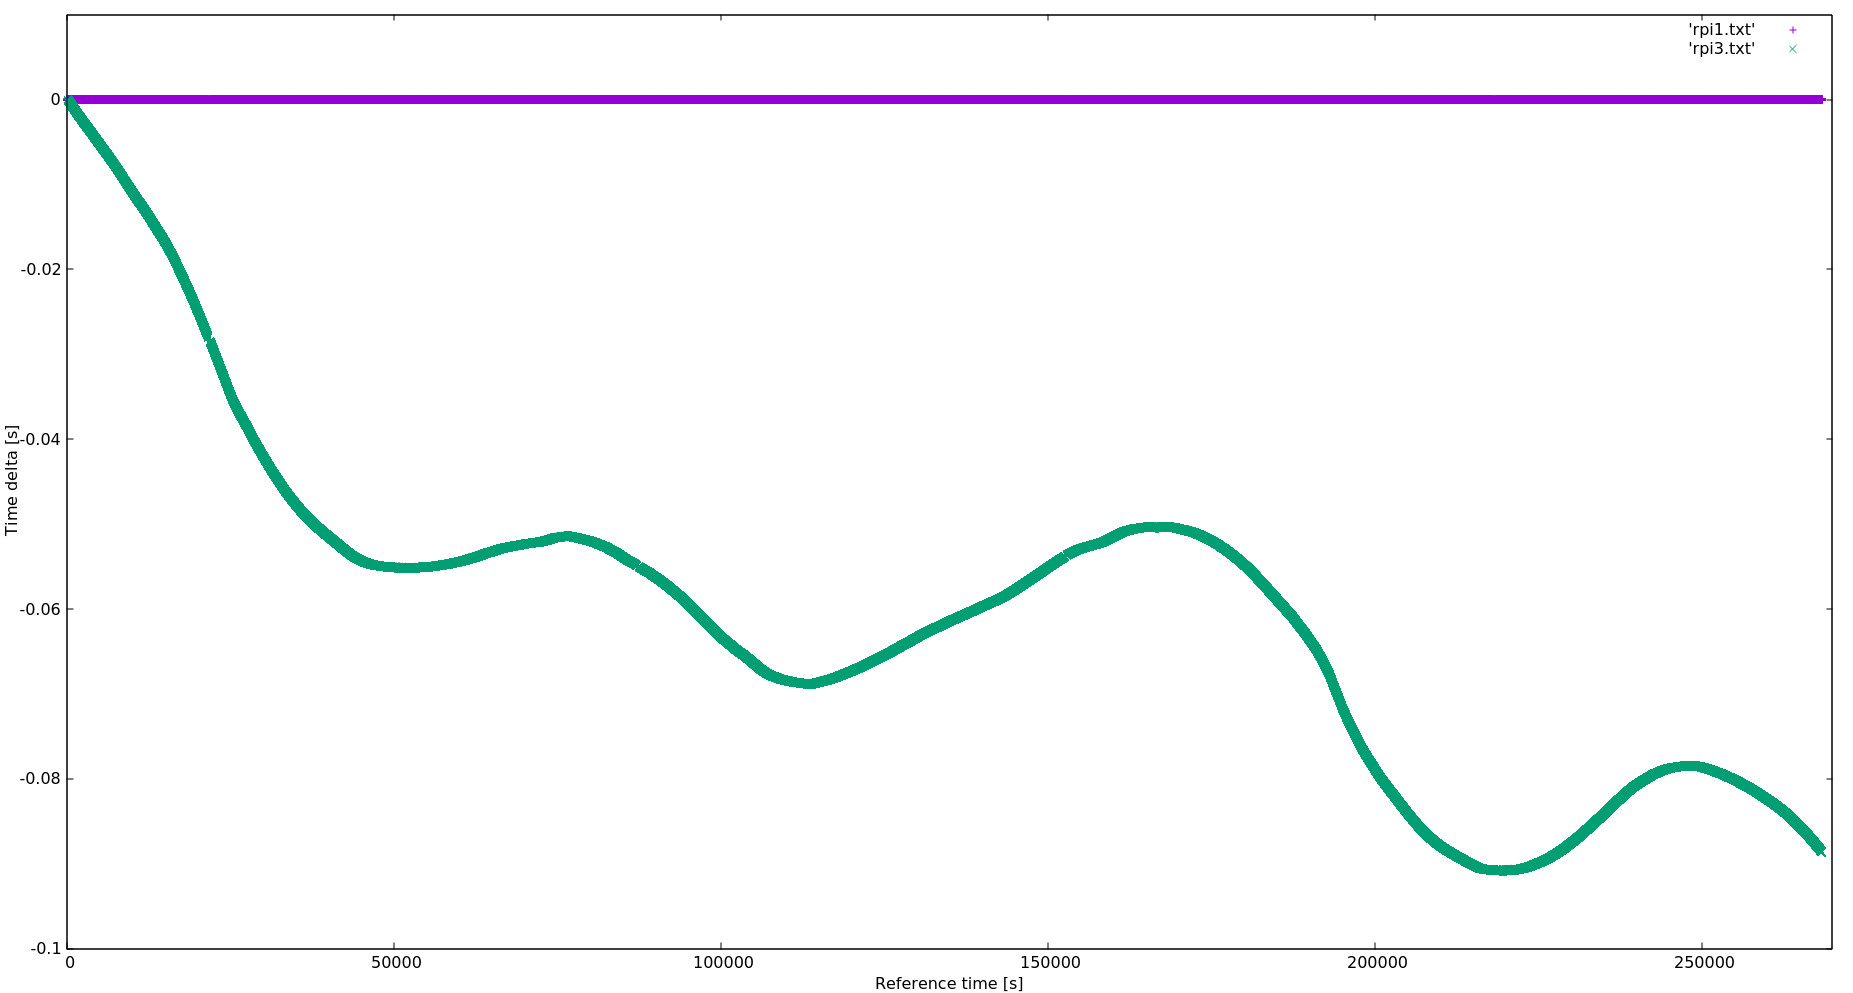
\includegraphics[width=1.0\textwidth]{figures/plot_nonlinear.png}
	\caption{Nonlinear deviation}
	\label{fig:plot_nonlinear}
\end{figure}

The reference clock \textit{rpi1} was synchronized by GPS while the clock of \textit{rpi3} was on its own. With about 3 days of measuring and the accompanying temperature fluctuations we can see that clock synchronization needs both: phase and frequency adjustment.
The measurement was started at 12:00 AM. We can see that the clock frequency is connected to the changing ambient temperature caused by the day cycle and weather.

\subsection{NTP}

The following measurement was taken with \textit{rpi1} as reference clock, \textit{rpi2} and \textit{rpi3} as synchronization targets.

\begin{figure}[H]
	\centering
	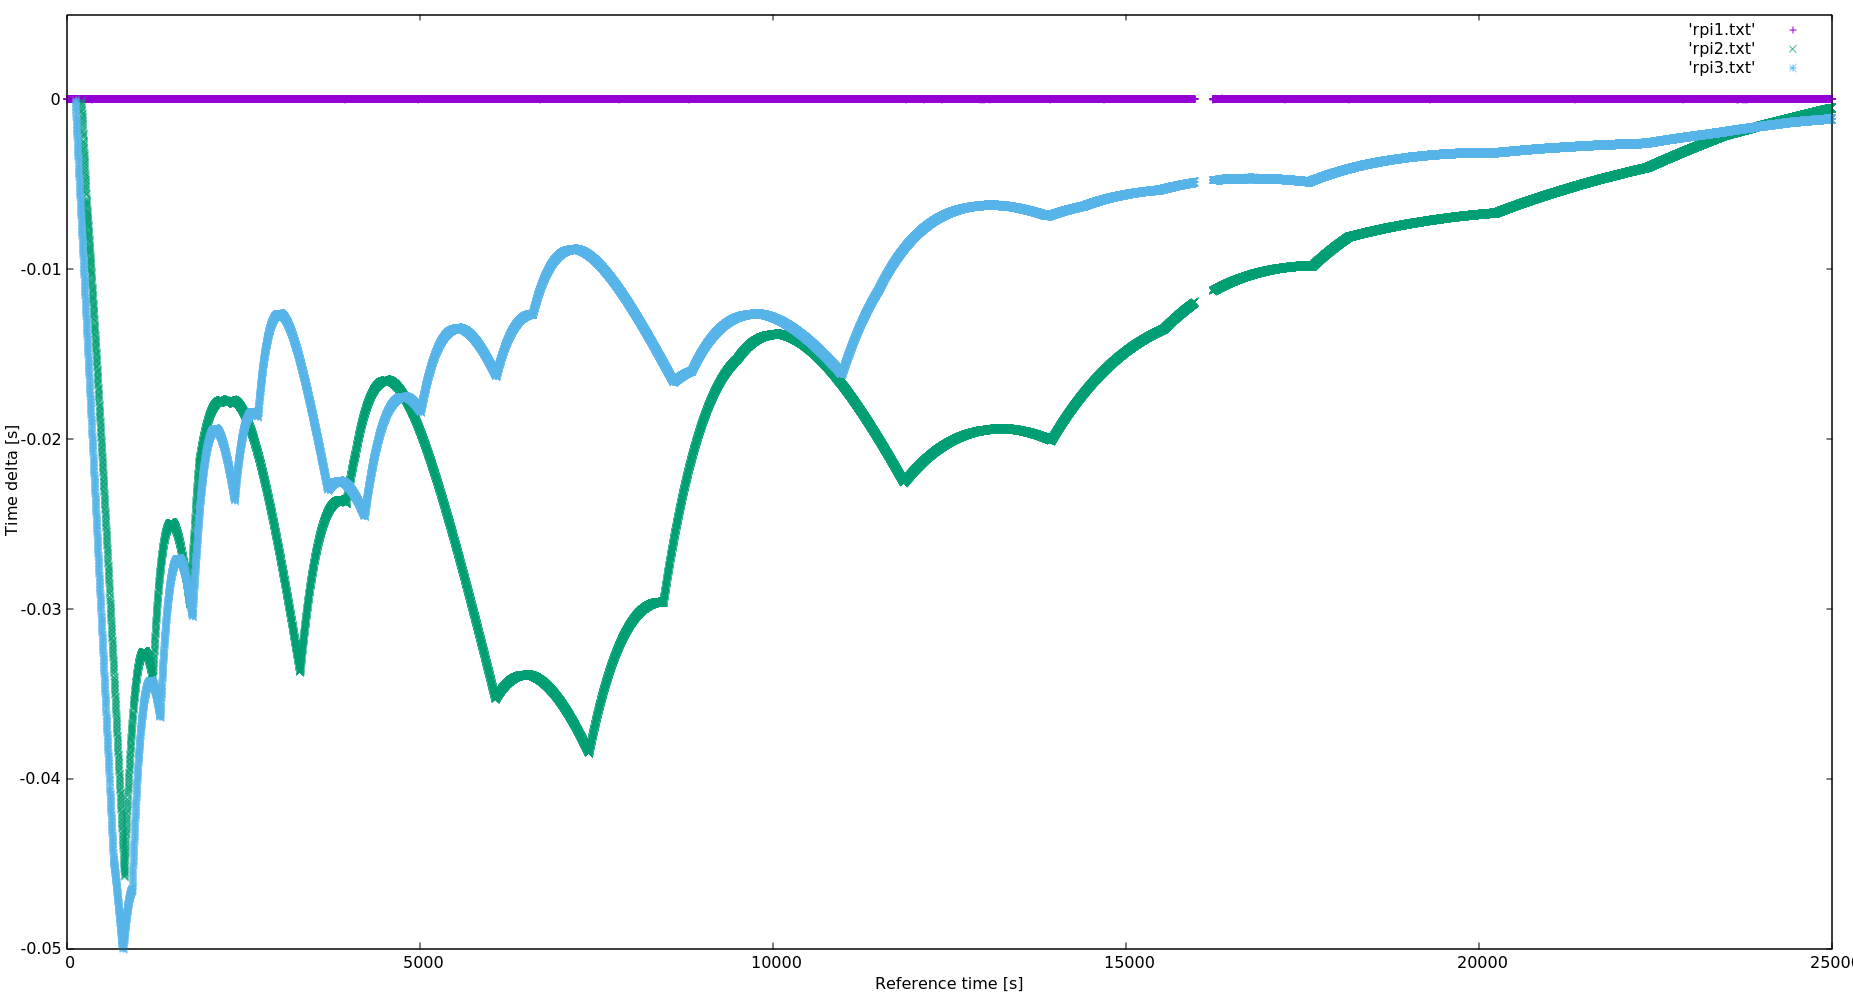
\includegraphics[width=1.0\textwidth]{figures/plot_ntp1.png}
	\caption{NTP synchronization}
	\label{fig:plot_ntp1}
\end{figure}

We can see the synchronization process in Figure \ref{fig:plot_ntp1}. With the initiation of the NTP daemon the target clock's phase is adjusted to about 0.1 ms relative to the reference clock. Then the frequency adjustment begins. In this case the target's clock frequency is very badly conditioned in comparison to the reference. NTP took about 14 h to fix this issue. Figure \ref{fig:plot_ntp2} shows the continuous time oscillation after the synchronization is done. This leads to an accuracy of about 0.2 ms.

\begin{figure}[H]
	\centering
	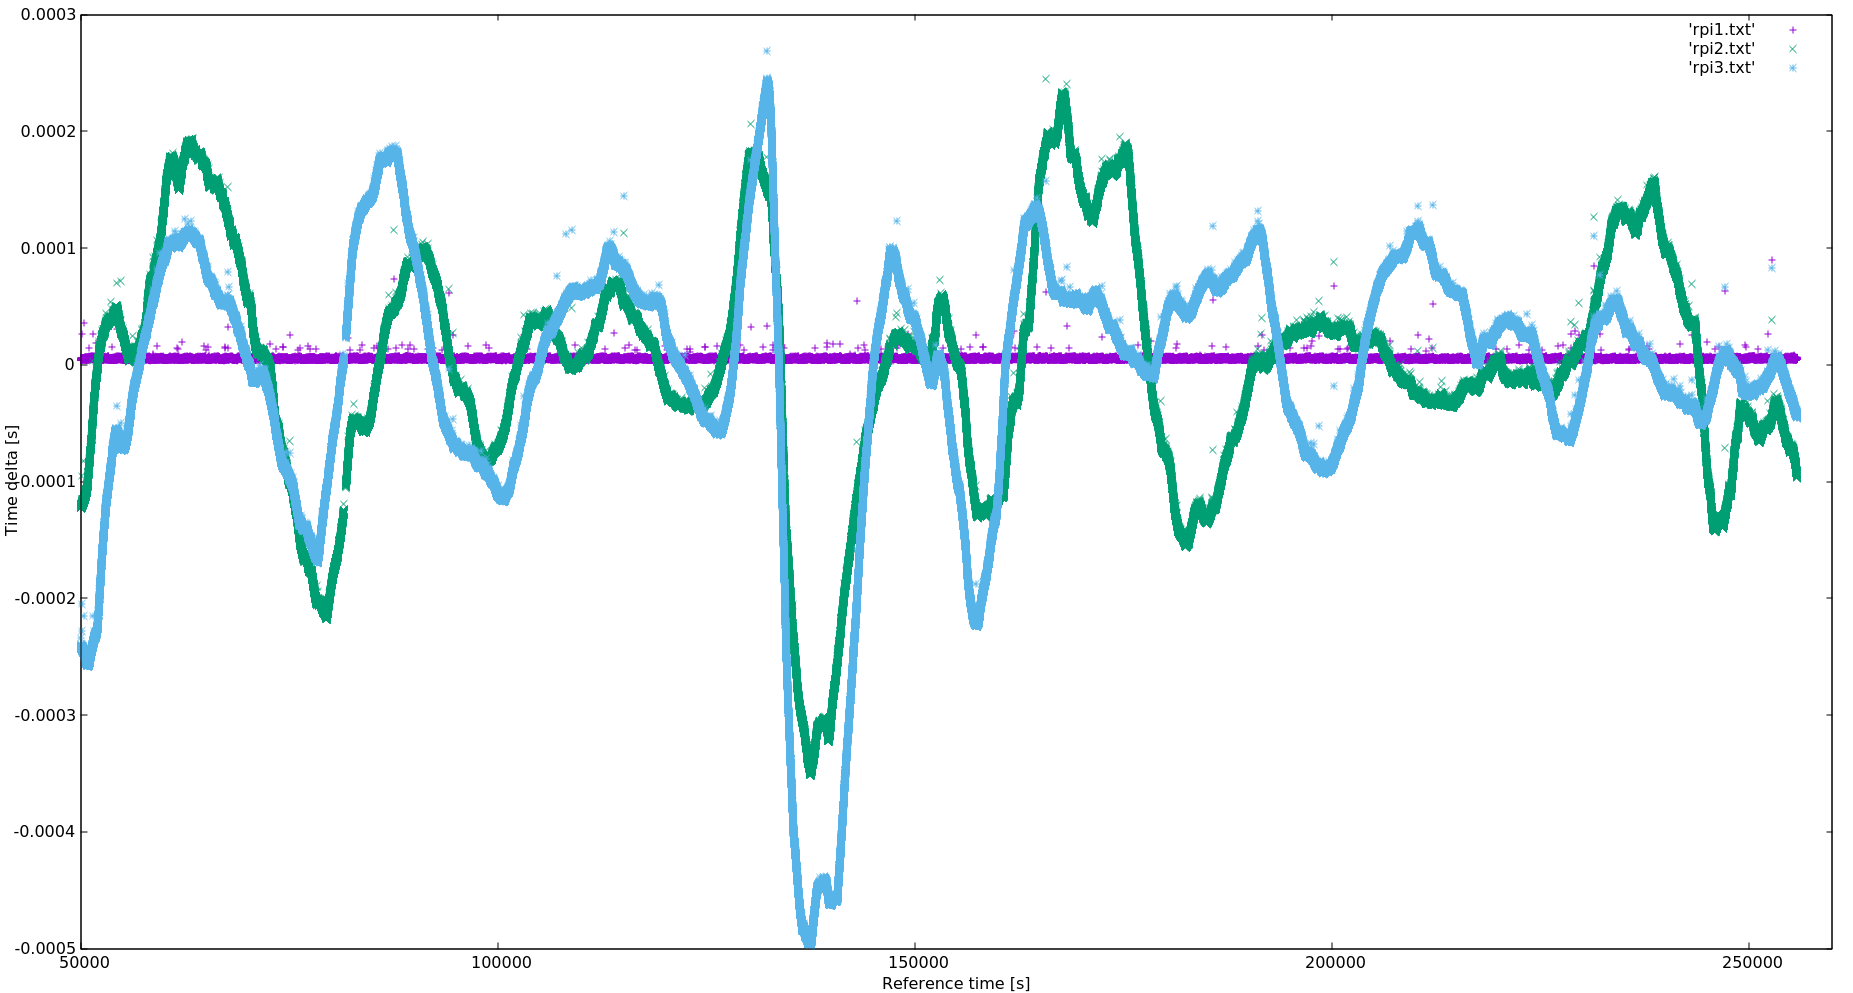
\includegraphics[width=1.0\textwidth]{figures/plot_ntp2.png}
	\caption{NTP accuracy}
	\label{fig:plot_ntp2}
\end{figure}

\subsection{PTP}

The topological setup is the same as before: \textit{rpi1} as reference clock, \textit{rpi2} and \textit{rpi3} as synchronization targets.

\begin{figure}[H]
	\centering
	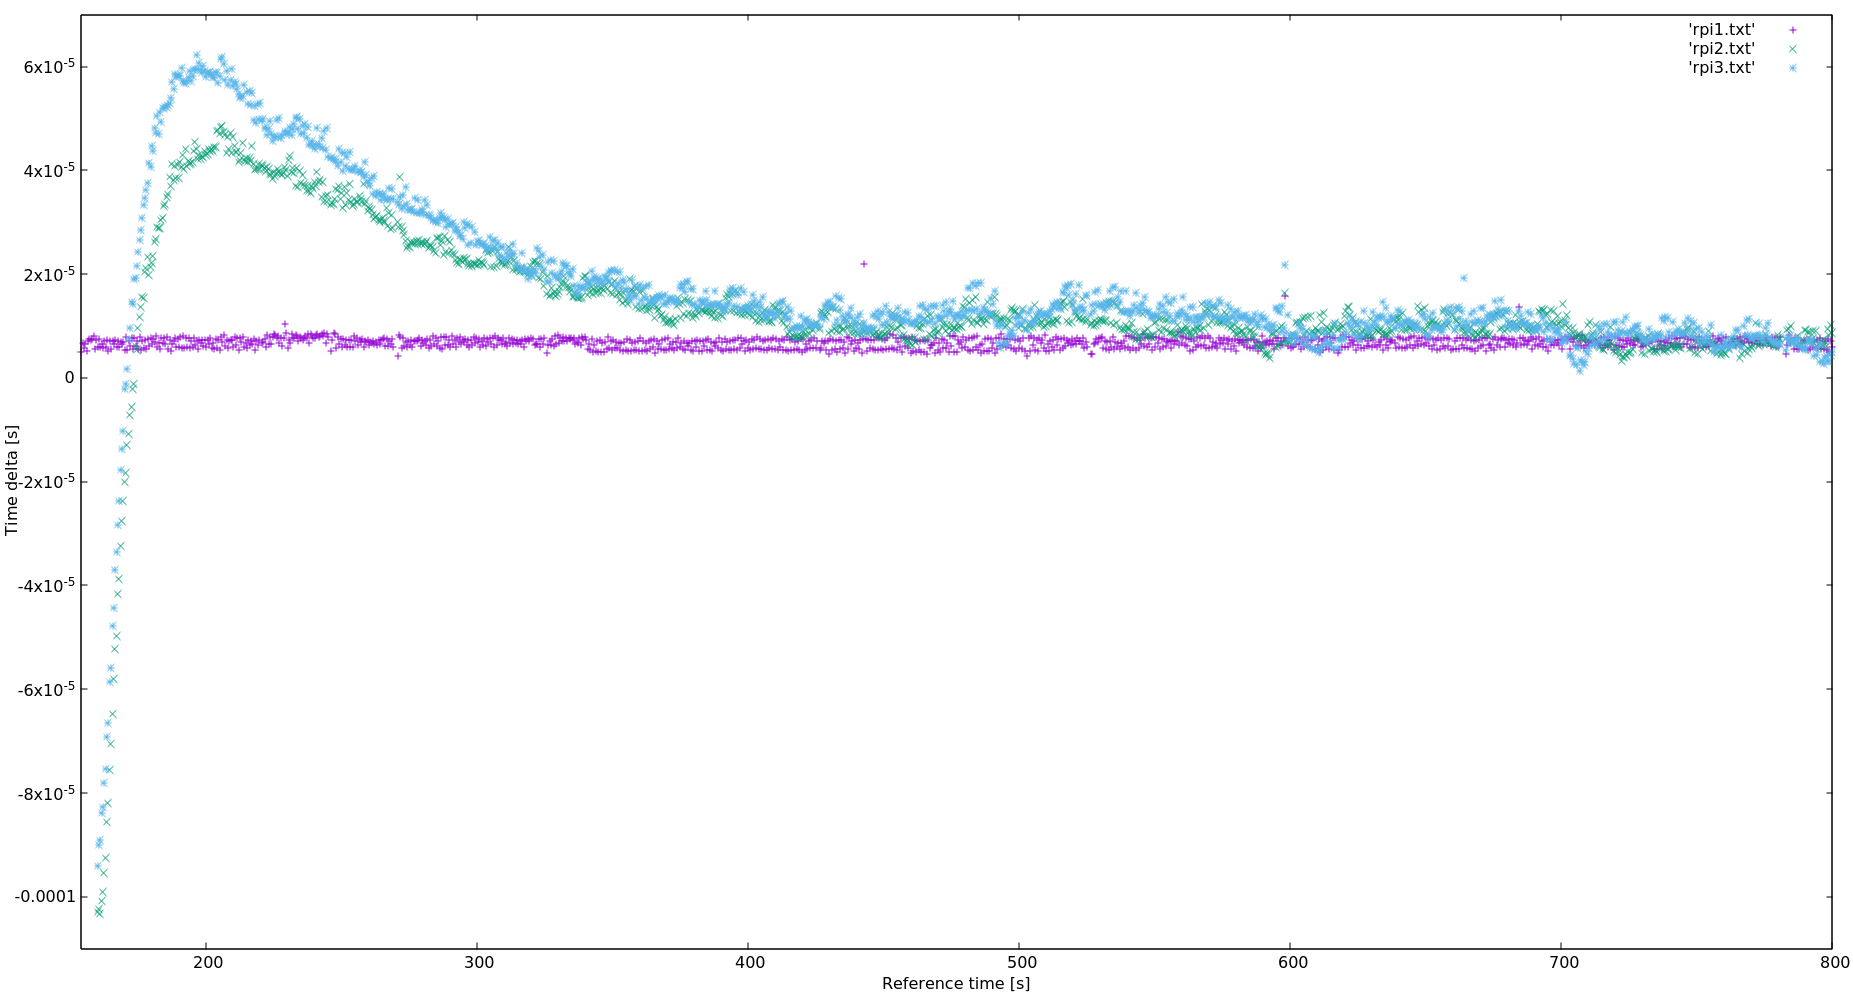
\includegraphics[width=1.0\textwidth]{figures/plot_ptp1.png}
	\caption{PTP synchronization}
	\label{fig:plot_ptp1}
\end{figure}

With the initiation of the PTP daemon the target's clock phase is adjusted to about 0.1 ms relative to the reference clock like shown in Figure \ref{fig:plot_ptp1}. The frequency adjustment takes over and completes in about 6 minutes. The accuracy gets very close to the measurement error with about 10 µs as we can see in Figure \ref{fig:plot_ptp2}.

\begin{figure}[H]
	\centering
	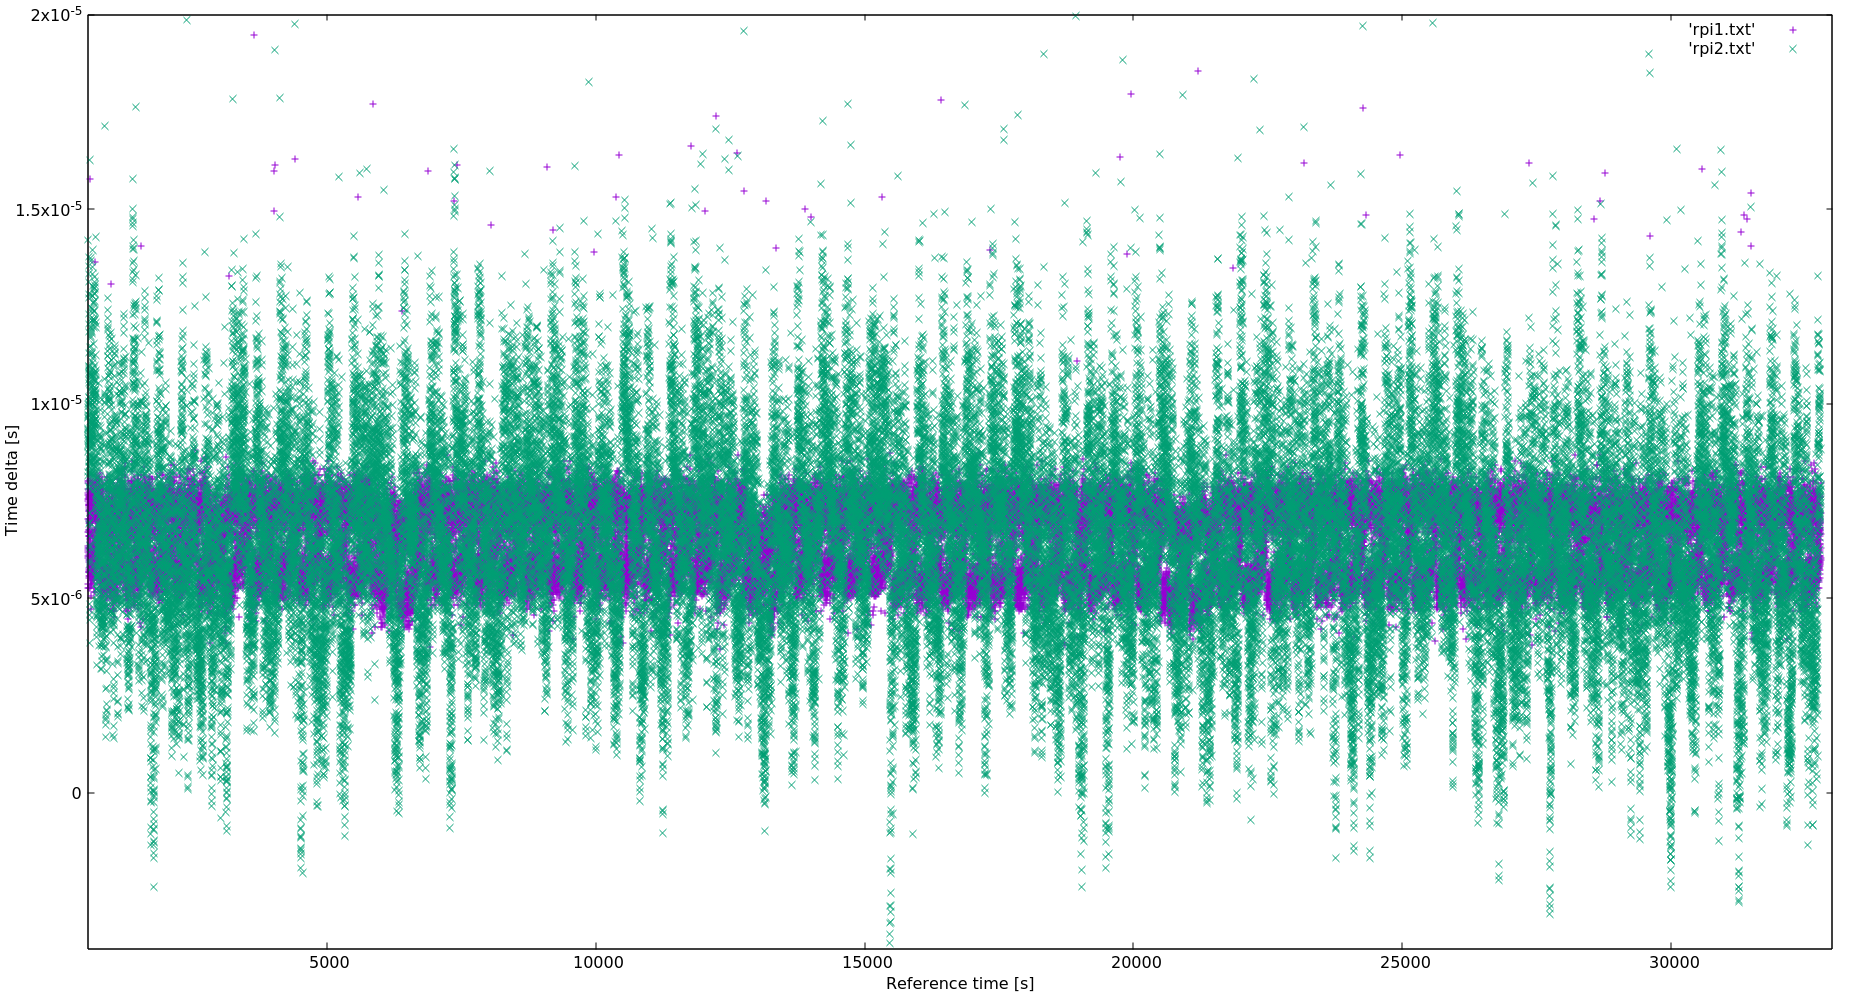
\includegraphics[width=1.0\textwidth]{figures/plot_ptp2.png}
	\caption{PTP accuracy}
	\label{fig:plot_ptp2}
\end{figure}

\subsection{GPS}

To get an estimate of the error, two GPS modules are required in order to compare them. \textit{rpi1} was started and synchronized long before \textit{rpi2}. With this way we have a stable reference to compare to and follow the initial time synchronization of \textit{rpi2}.

\begin{figure}[H]
	\centering
	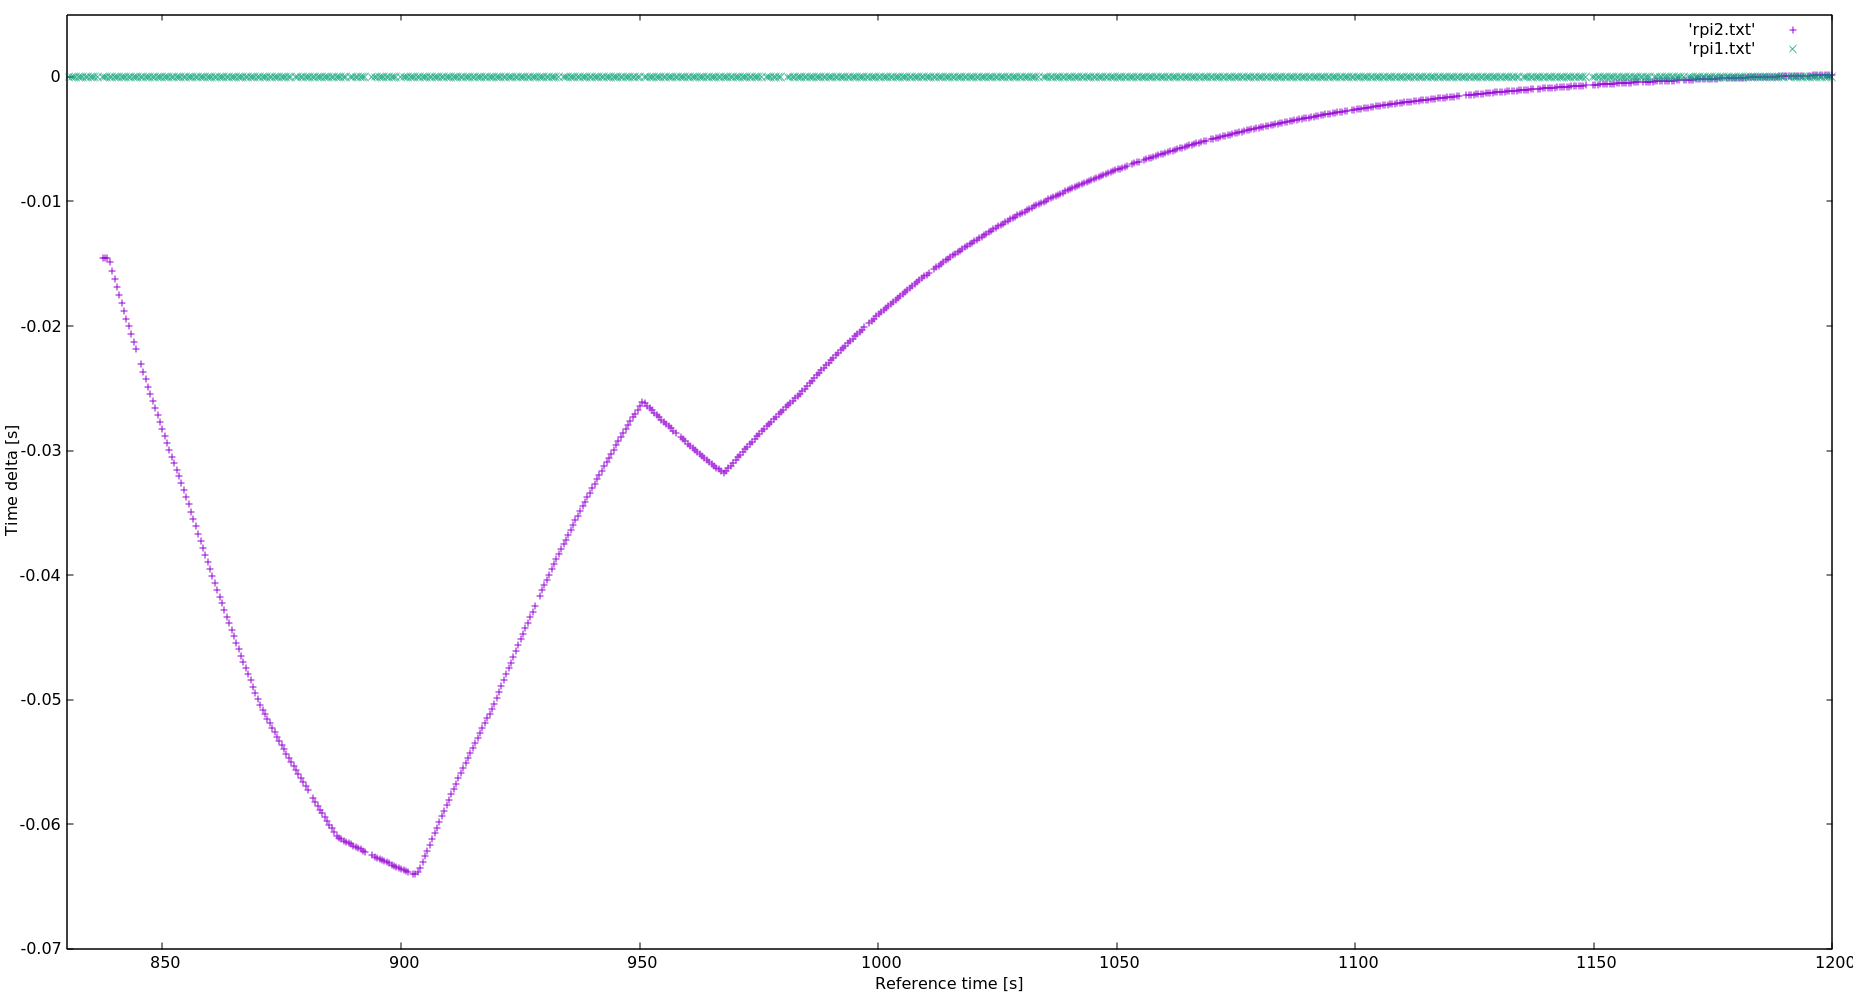
\includegraphics[width=1.0\textwidth]{figures/plot_gps1.png}
	\caption{GPS synchronization}
	\label{fig:plot_gps1}
\end{figure}

\begin{figure}[H]
	\centering
	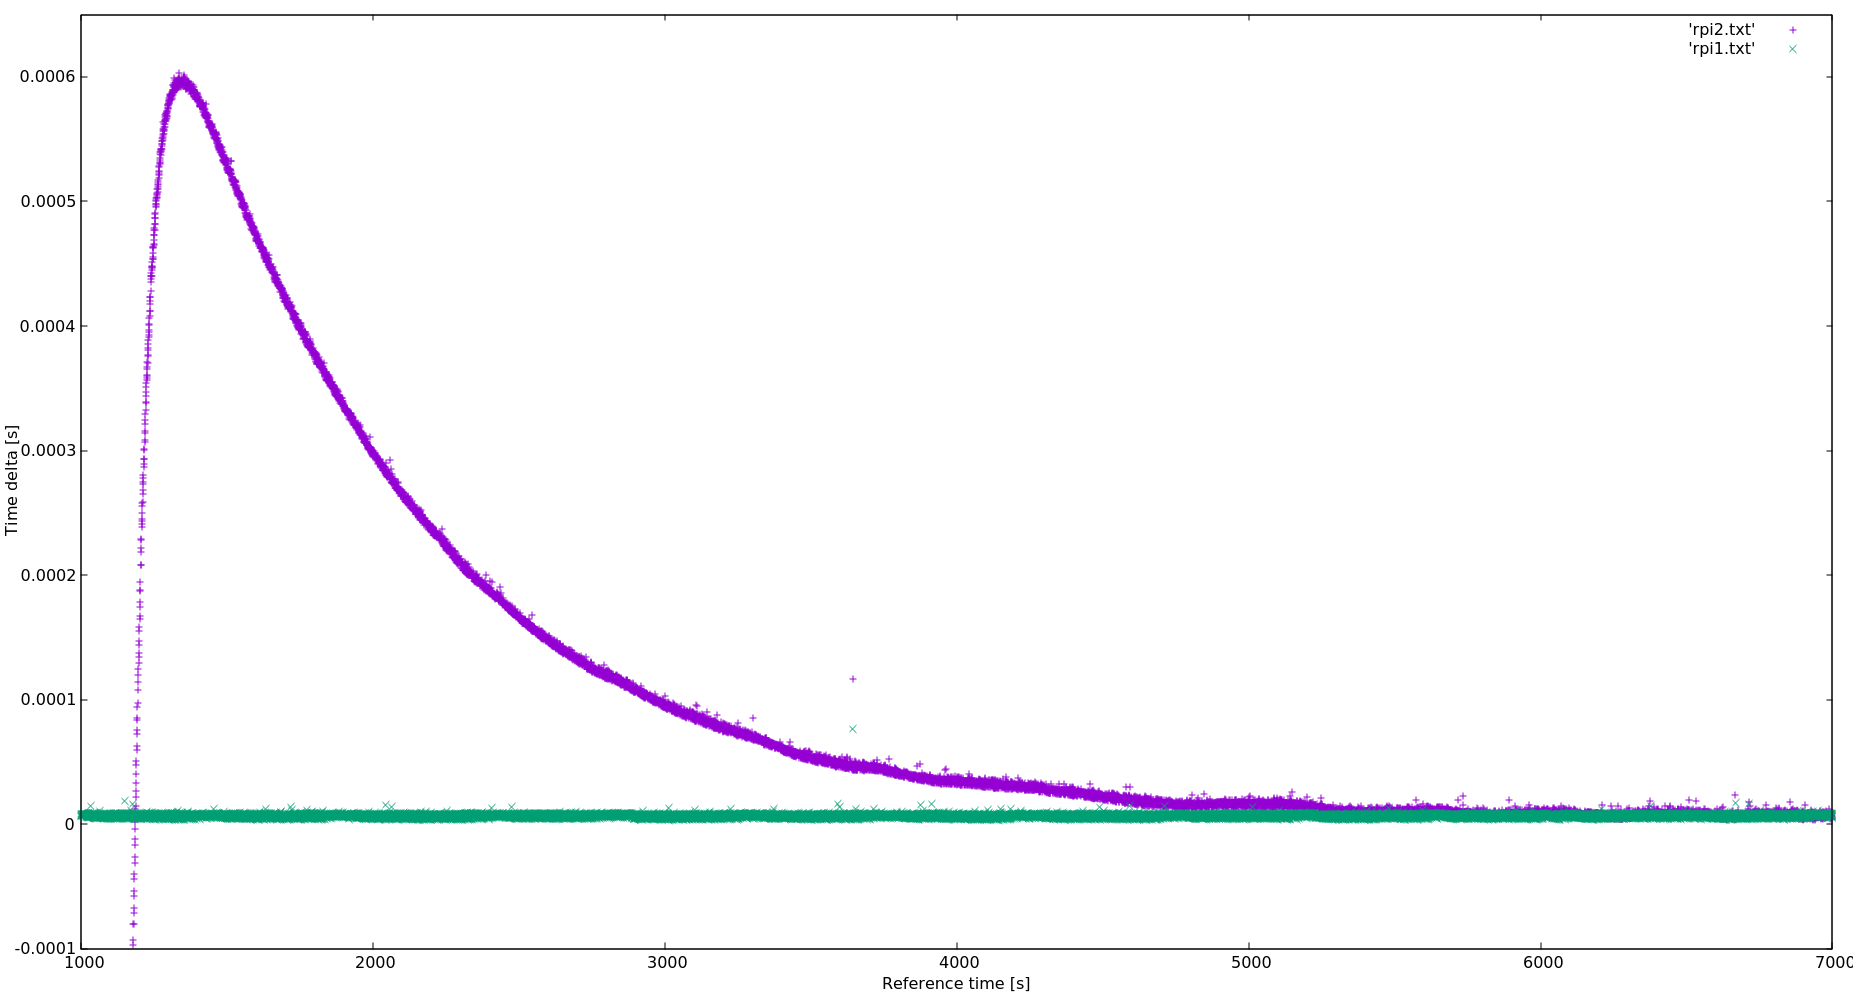
\includegraphics[width=1.0\textwidth]{figures/plot_gps2.png}
	\caption{GPS synchronization close-up}
	\label{fig:plot_gps2}
\end{figure}

The initiation of the NTP daemon with GPS configuration adjusts the phase to about 10 ms relative to the reference clock like shown in Figure \ref{fig:plot_gps1}. The high error comes from the serial connection. NTP starts using the serial interface first and heads over to PPS after analyzing the signal. After about 2 minutes the PPS signal gets accepted, followed by a slow converging curve towards reference within about 90 minutes shown in Figure \ref{fig:plot_gps2}.

\begin{figure}[H]
	\centering
	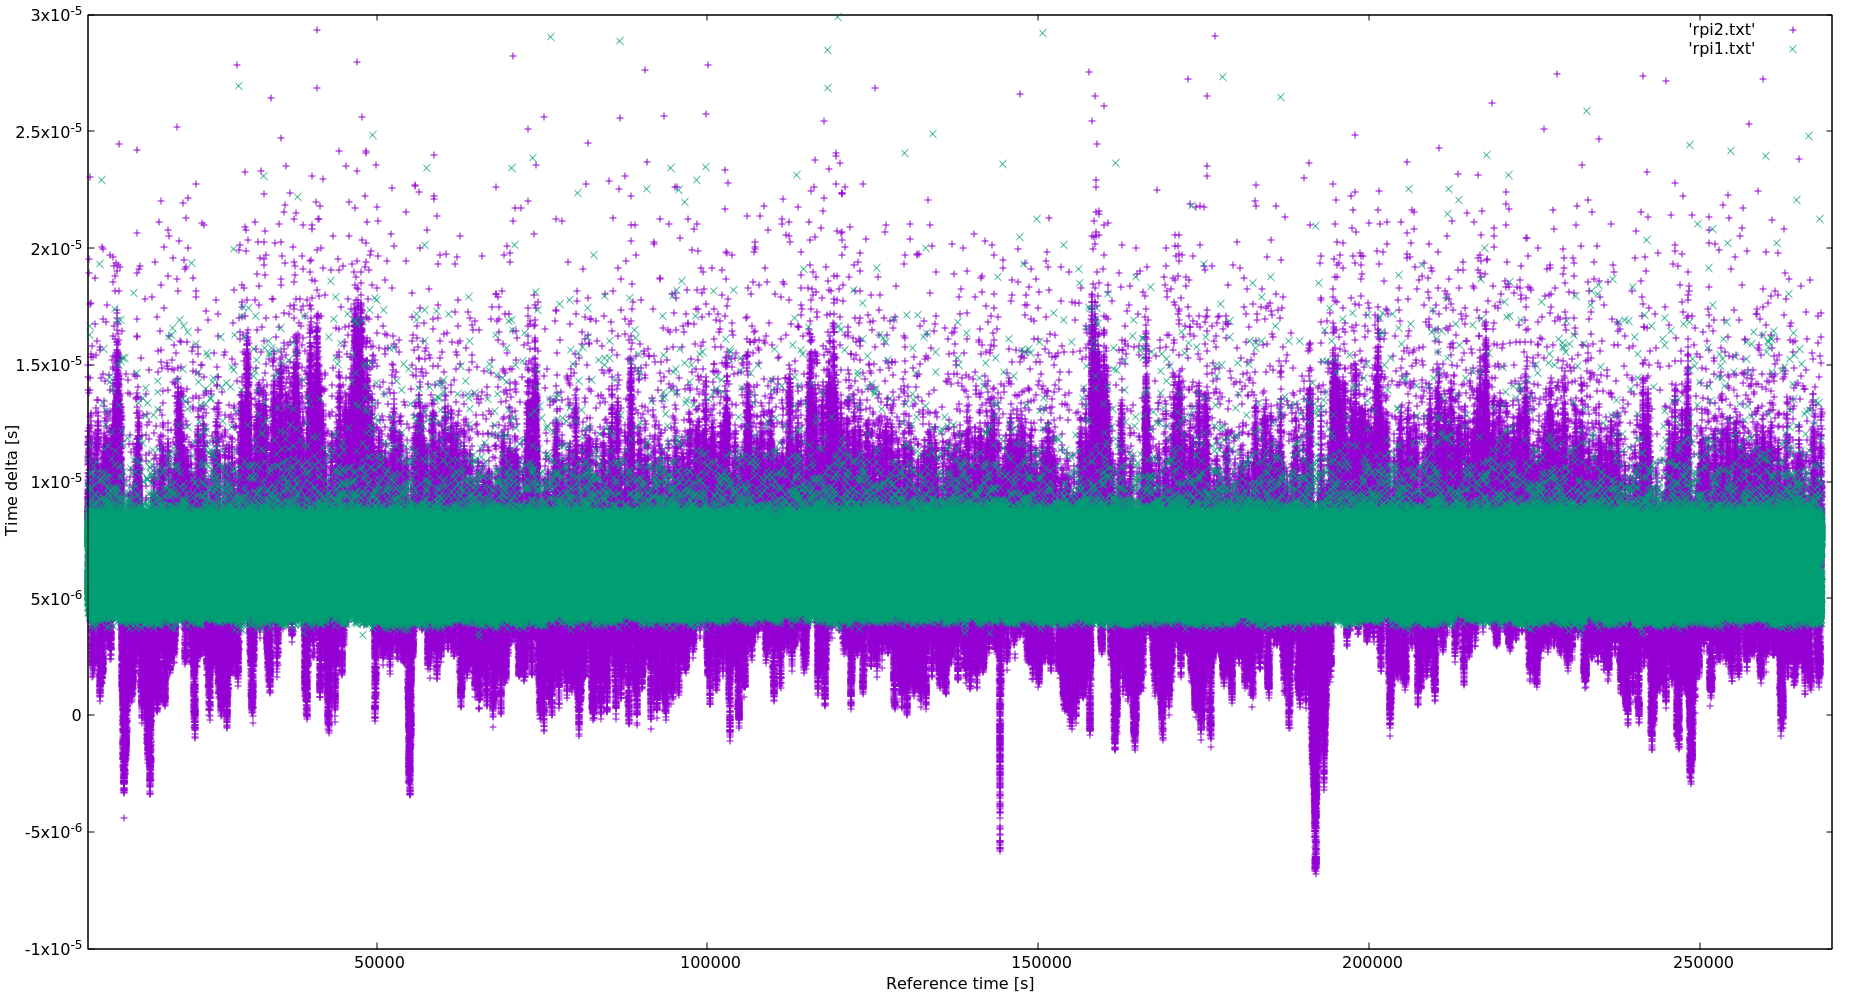
\includegraphics[width=1.0\textwidth]{figures/plot_gps3.png}
	\caption{GPS accuracy}
	\label{fig:plot_gps3}
\end{figure}

In the end we reach an accuracy close to the measurement error of about 10 µs illustrated by Figure \ref{fig:plot_gps3}.



\chapter{Conclusion}
\label{ch:conclusion}
The delay measurements made clear that, at least for version 4.6.7, the mainline kernel is the better option in terms of latency if higher outliers are acceptable. Besides, the dynamic CPU frequency stepping has a similar disadvantage and should be avoided if the power consumption isn’t that relevant.

For time synchronization in a local switched network PTP is the best choice. It has the fastest convergence and the accuracy is comparable to GPS. If the absolute time should be accurate is required, a GPS module as PTP source would be the best solution. While GPS converges in about 90 minutes, the target clocks would have already completed the synchronization process and keep the 10 µs accuracy to the time source.



\cleardoublepage
\pagenumbering{roman} \setcounter{page}{1}
\printbibliography

\appendix

\chapter{Kernel compilation}
\label{ap:kernel}
\begin{lstlisting}[label=lst:kernel, language=bash, caption=Kernel compilation]
# create kernel directory
mkdir -p tmp/boot
mkdir -p tmp/lib/modules

# get the cross compilation toolchain
git clone https://github.com/raspberrypi/tools.git
export ARCH=arm
export CROSS_COMPILE=$(pwd)/tools/arm-bcm2708/gcc-linaro-arm-linux-gnueabihf-raspbian/bin/arm-linux-gnueabihf-
export INSTALL_MOD_PATH=$(pwd)/tmp/lib/modules

# get the kernel source
git clone https://github.com/raspberrypi/linux.git
cd linux
git checkout rpi-4.6.y

# for PREEMPT_RT continue here
# first have a look at the Makefile. VERSION, PATCHLEVEL, and SUBLEVEL define the kernel version.
wget https://www.kernel.org/pub/linux/kernel/projects/rt/4.6/patch-4.6.7-rt14.patch.gz
zcat patch-4.6.7-rt14.patch.gz | patch -p1
rm patch-4.6.7-rt14.patch.gz
# resolve any upcoming conflicts
# PREEMPT_RT done

# configure the kernel
export KERNEL=kernel7
make bcm2709_defconfig
# enable CONFIG_PREEMPT_RT_FULL and HIGH_RES_TIMERS
make menuconfig

# compile
make zImage
make modules
make dtbs
make modules_install

# pack the kernel
cd ..
linux/scripts/mkknlimg linux/arch/arm/boot/zImage tmp/boot/$KERNEL.img
cp linux/arch/arm/boot/dts/*.dtb tmp/boot/
cp -r linux/arch/arm/boot/dts/overlays tmp/boot
cd tmp
tar -czf ../kernel.tar.gz *
\end{lstlisting}

\section{Kernel module compilation}

\begin{lstlisting}[label=lst:kernel_module, language=bash, caption=Kernel module compilation]
git clone https://github.com/andiwand/gpio-netlink.git
cd gpio-netlink
# set the following variables appropriately
# CCPREFIX is used for cross compilation
# KERNEL_SRC points to the compiled kernel source directory
CCPREFIX=$(pwd)/../tools/arm-bcm2708/gcc-linaro-arm-linux-gnueabihf-raspbian/bin/arm-linux-gnueabihf- KERNEL_SRC=$(pwd)/../linux make
\end{lstlisting}


\chapter{GPS configuration}
\label{ap:gps}
\section{Wiring}

\begin{center}
    \begin{tabular}{ | l | l | }
    \hline
    \textbf{Ultimate GPS Breakout v3} & \textbf{Raspberry Pi 3} \\ \hline
    VIN & Any 3V3 or 5V \\ \hline
    GND & Any ground \\ \hline
    TX & Pin 10 | GPIO 15 | UART0\_RXD \\ \hline
    RX & Pin  8 | GPIO 14 | UART0\_TXD \\ \hline
    PPS & Pin 12 | GPIO 12 | PCM\_CLK \\ \hline
    \end{tabular}
\end{center}

\section{GPS configuration}

\begin{lstlisting}[label=lst:gps, language=bash, caption=GPS configuration]
# install requirements
apt-get install picocom pps-tools
apt-get install gpsd gpsd-clients python-gps

vim /boot/config.txt
### remove lines:
console=serial0,115200
### add lines:
# gps
dtoverlay=pps-gpio,gpiopin=18
enable_uart=1

echo "pps-gpio" >> /etc/modules

# configure pps dev files
echo -n '' > /etc/udev/rules.d/10-pps.rules
echo 'KERNEL=="ttyS0", SYMLINK+="gps0"' >> /etc/udev/rules.d/10-pps.rules
echo 'KERNEL=="pps0", OWNER="root", GROUP="tty", MODE="0660", SYMLINK+="gpspps0"' >> /etc/udev/rules.d/10-pps.rules

# configure gpsd
echo -n '' > /etc/default/gpsd
echo 'START_DAEMON="true"' >> /etc/default/gpsd
echo 'GPSD_OPTIONS="-n"' >> /etc/default/gpsd
echo 'DEVICES="/dev/gps0"' >> /etc/default/gpsd
echo 'USBAUTO="false"' >> /etc/default/gpsd

# compile ntp with pps and gps support
cd /usr/src
wget http://archive.ntp.org/ntp4/ntp-4.2/ntp-4.2.8p8.tar.gz
tar -zxvf ntp-4.2.8p8.tar.gz
cd ntp-4.2.8p8
./configure
make && make install
\end{lstlisting}


\chapter{Measurement environment}
\label{ap:environment}
\begin{lstlisting}[label=lst:env, language=bash, caption=Measurement environment]
# install requirements
apt install build-essential libnuma-dev
apt install vim git screen adjtimex ptpd
apt install python python-pip python3 python3-pip

# update pip
pip2 install --upgrade pip setuptools
pip3 install --upgrade pip setuptools

# disable services
systemctl stop ntp
systemctl stop ptpd
systemctl disable ntp
systemctl disable ptpd

vim /boot/config.txt
### add lines
# static frequency
force_turbo=1
boot_delay=1
arm_freq=800
arm_freq_min=800

vim /etc/dhcp/dhclient.conf
### remove "ntp-servers" from "requests"

# install cyclictest
git clone git://git.kernel.org/pub/scm/utils/rt-tests/rt-tests.git
cd rt-tests
git checkout stable/v1.0
make cyclictest
cd ..

# install custom tools
pip3 install https://github.com/andiwand/time-config/archive/master.zip
pip3 install https://github.com/andiwand/time-experiments/archive/master.zip
git clone https://github.com/andiwand/time-experiments.c.git && cd time-experiments.c && make && cd ..
git clone https://github.com/andiwand/time-tools.git
pip3 install https://github.com/andiwand/time-analysis/archive/master.zip

# copy the gpio-netlink kernel module into the current directory
\end{lstlisting}


\end{document}
